%  LaTeX support: latex@mdpi.com
%  In case you need support, please attach any log files that you could have, and specify the details of your LaTeX setup (which operating system and LaTeX version / tools you are using).

%=================================================================

% LaTeX Class File and Rendering Mode (choose one)
% You will need to save the "mdpi.cls" and "mdpi.bst" files into the same folder as this template file.

%=================================================================

\documentclass[remotesensing,article,accept,moreauthors,pdftex,12pt,a4paper]{mdpi} 
%--------------------
% Class Options:
%--------------------
% journal
%----------
% Choose between the following MDPI journals:
% actuators, administrativesciences, aerospace, agriculture, agronomy, algorithms, animals, antibiotics, antibodies, antioxidants, appliedsciences, arts, atmosphere, atoms, axioms, behavioralsciences, bioengineering, biology, biomedicines, biomolecules, biosensors, brainsciences, buildings, cancers, catalysts, cells, challenges, chemosensors, children, chromatography, climate, coatings, computation, computers, cosmetics, crystals, dentistryjournal, diagnostics, diseases, diversity, econometrics, economies, education, electronics, energies, entropy, environmentalsciences, environments, fibers, foods, forests, futureinternet, galaxies, games, genes, geosciences, healthcare, humanities, informatics, information, inorganics, insects, ijerph, ijfs, ijms, ijgi, jcdd, jcm, jdb, jfb, joi, jlpea, jmse, jpcg, jpm, jrfm, jsan, land, laws, life, lubricants, machines, marinedrugs, materials, mathematics, medicalsciences, membranes, metabolites, metals, microarrays, micromachines, microorganisms, minerals, molbank, molecules, nanomaterials, ncrna, nutrients, pathogens, pharmaceuticals, pharmaceutics, pharmacy, photonics, plants, polymers, processes, proteomes, publications, religions, remotesensing, resources, risks, robotics, sensors, socialsciences, societies, sports, sustainability, symmetry, systems, technologies, toxics, toxins, vaccines, veterinarysciences, viruses, water
%---------
% article
%---------
% The default type of manuscript is article, but could be replaced by using one of the class options: 
% article, review, communication, commentary, bookreview, correction, addendum, editorial, changes, supfile, casereport, comment, conceptpaper, conferencereport, meetingreport, discussion, essay, letter, newbookreceived, opinion, projectreport, reply, retraction, shortnote, technicalnote, creative
%----------
% submit
%----------
% The class option "submit" will be changed to "accept" by the Editorial Office when the paper is accepted. This will only make changes to the frontpage (e.g. the logo of the journal will get visible), the headings, and the copyright information. Journal info and pagination for accepted papers will also be assigned by the Editorial Office.
% Please insert a blank line is before and after all equation and eqnarray environments to ensure proper line numbering when option submit is chosen
%------------------
% moreauthors
%------------------
% If there is only one author the class option oneauthor should be used. Otherwise use the class option moreauthors.
%---------
% pdftex
%---------
% The option "pdftex" is for use with pdfLaTeX only. If eps figure are used, use the optioin "dvipdfm", with LaTeX and dvi2pdf only.

%=================================================================
\setcounter{page}{1}
\lastpage{x}
\doinum{10.3390/------}
\pubvolume{xx}
\pubyear{2014}
\history{Received: xx / Accepted: xx / Published: xx}
%------------------------------------------------------------------
% The following line should be uncommented if the LaTeX file is uploaded to arXiv.org
%\pdfoutput=1

%=================================================================

% Add packages and commands to include here
% The amsmath, amsthm, amssymb, hyperref, caption, float and color packages are loaded by the MDPI class.
%\usepackage{graphicx}
%\usepackage{subfigure,psfig}


\usepackage{xcolor}
\usepackage{graphicx}
\usepackage{subcaption} 
\usepackage{url}
\usepackage{multirow}
\usepackage{amsmath}
\usepackage{amssymb}
\usepackage{rotating}




\usepackage[T1]{fontenc}
\usepackage{array}
\usepackage{makecell}
\newcolumntype{x}[1]{>{\centering\arraybackslash}p{#1}}
\usepackage{tikz}
\newcommand\diag[4]{%
  \multicolumn{1}{p{#2}|}{\hskip-\tabcolsep
  $\vcenter{\begin{tikzpicture}[baseline=0,anchor=south west,inner sep=#1]
  \path[use as bounding box] (0,0) rectangle (#2+2\tabcolsep,\baselineskip);
  \node[minimum width={#2+2\tabcolsep-\pgflinewidth},
        minimum  height=\baselineskip+\extrarowheight-\pgflinewidth] (box) {};
  \draw[line cap=round] (box.north west) -- (box.south east);
  \node[anchor=south west] at (box.south west) {#3};
  \node[anchor=north east] at (box.north east) {#4};
 \end{tikzpicture}}$\hskip-\tabcolsep}}



\newcommand\red[1]{\textcolor{red}{#1}} % Red marker to declare errors.

%=================================================================
%% Please use the following mathematics environments:
%\theoremstyle{mdpi}
%\newcounter{thm}
%\setcounter{thm}{0}
%\newcounter{ex}
%\setcounter{ex}{0}
%\newcounter{re}
%\setcounter{re}{0}
%\newtheorem{Theorem}[thm]{Theorem}
%\newtheorem{Lemma}[thm]{Lemma}
%\newtheorem{Characterization}[thm]{Characterization}
%\newtheorem{Proposition}[thm]{Proposition}
%\newtheorem{Property}[thm]{Property}
%\newtheorem{Problem}[thm]{Problem}
%\newtheorem{Example}[ex]{Example}
%\newtheorem{Remark}[re]{Remark}
%\newtheorem{Corollary}[thm]{Corollary}
%\newtheorem{Definition}[thm]{Definition}
%% For proofs, please use the proof environment (the amsthm package is loaded by the MDPI class).

%=================================================================

% Full title of the paper (Capitalized)
\Title{An Empirical Study of Atmospheric Corrections Impacts on Hyperspectral Classification of Savanah Tree Species Using $k$-fold Cross-Validated Non-linear SVM}

% Authors (Add full first names)
\Author{Morteza Shahriari Nia $^{1,}$*, Daisy Zhe Wang $^{1}$, Milenko Petrovic $^{2}$, Stephanie Ann Bohlman $^{3}$ and Paul Gader $^{1}$}

% Affiliations / Addresses (Add [1] after \address if there is only one affiliation.)
\address{%
$^{1}$ Department of Computer and Information Science and Engineering, University of Florida, 432 Newell Dr., Gainesville, Florida 32611, USA\\
$^{2}$ Institute for Human and Machine Cognition, 15 SE Osceola Ave, Ocala, Florida 34471, USA\\
$^{3}$ School of Forest Resources and
Conservation, 349 Newins Ziegler Hall, Gainesville, Florida
32611, USA}

% Contact information of the corresponding author (Add [2] after \corres if there are more than one corresponding author.)
\corres{msnia@cise.ufl.edu}

% Abstract (Do not use inserted blank lines, i.e. \\) 
\abstract{Identifying savannah species at ecological scale is a key step in measuring biomass, carbon reserves, drought and invasive species spread predictions. 
In this paper we perform classification and geo-mapping of tree species from hyperspectral imagery collected using AVIRIS airborne sensors at pixel level. 
We provide a thorough comparison of the effects of ATCOR and FLAASH atmospheric corrections in prediction accuracy. 
We exploit Gaussian Filters to eliminate sensor measurements and calibration errors, to the best of our knowledge we are the first in employing Gaussian Filters for hyperspectral species classification. 
This is a pilot study for NEON in Ordway-Swisher Biological Station in north-central Florida. 
Among indexes we found that applying NDVI and NIR wavelength (734.1$ n m$) threshold filters do not play constructive roles in SVM model performance for species classification. 
We observed that removal of water absorption bands to be most helpful.  
Species classification was performed using variety of Support Vector Machine kernels where Radial Basis outperformed others. 
Our classification produces accurate predictions of about 75\%. 
}

% Keywords: add 3 to 10 keywords
\keyword{Species classification; Hyperspectral; High spatial and spectral resolution; Pixel-level classification; Support Vector Machines; Ordway-Swisher Biological Station;  National Ecological Observatory Network; Airborne Observation Platform protocols;} % NEON-AOP

% The fields PACS, MSC, and JEL may be left empty or commented out if not applicable
%\PACS{}
%\MSC{}
%\JEL{}

\begin{document}

\section{Introduction}




Mapping tree species by remote sensing techniques is an essential step in understanding how planetrary species play roles at ecological scale. 
This will enable us to study land covers, climate change, invasive species, plant competitions, predict fire potentials and spreading routes, soil characteristics and etc \cite{scholes1997tree, colgan2012mapping}. This kind of research has only been possible via the technological advancements in remote sensing facilities such as hyperspectral imagery or Light Detection and Ranging (LiDAR). 
Various studies have dealt with identifying tree species at both pixel level and crown level and as technology becomes available and economically feasible, studies tend to cover larger areas. 
Carnegie Airborne Observatory\footnote{http://cao.stanford.edu/} (CAO)  is a major pioneer in employing airborne technology for remote sensing at ecology scale where they study large areas in Amazonians, Kruger National Park in South Africa, Madagascar among others.
 Colgan et al. \cite{colgan2012mapping} uses a two stage Support Vector Machines (SVM) at pixel level and at crown level for tree species classification where LiDAR measurements were used for crown segmentation. 
 F\'{e}ret and Asner \cite{feret2013tree} study the accuracy of various parametric/non-parametric supervised classification techniques and observed that there is a clear advantage in using Regularized Discriminant Analysis, Linear Discriminant Analysis, and Support Vector Machines among others. 



Cho et al. \cite{cho2012mapping} compares accuracies when different hyperspectral sensors of CAO, WorldView2 and QuickBird are utilized by convolving the 72 bands of CAO to eight and four multispectral channels available in the WorldView-2 and Quickbird satellite sensors, respectively. 
Interestingly enough they observed that WorldView-2 produced more accurate classification results then QuickBird and finally CAO. 
Clark et al. takes on another perspective and compares lab measurements to pixel and to crown level and try to identify important wavelength regions for species discrimination \cite{clark2005hyperspectral}. 
They observed that optimal regions of the spectrum for species discrimination varied with scale. However, near-infrared (700-1327$nm$) bands were consistently important regions across all scales. 
Bands in the visible region (437-700$nm$) and shortwave infrared (1994-2435$nm$) were more important at pixel and crown scales  \cite{clark2005hyperspectral}. 
Clark et al. in another work evaluates the effects of different metrics used for classification (indexes, derivatives, signals themselves and all together) \cite{clark2012species}. 
There are other tree species classification works such as \cite{dalponte2014tree, feret2012semi, feret2013tree, ghosh2014framework, immitzer2012tree, naidoo2012classification, ustin2009retrieval} that share the same approach with minor variations. 

There are other schools of thought that try to identify more context specific features of remote rensing. 
For example Baldeck and Asner \cite{baldeck2013estimating} try to measure how similar beta diversity of regions are; 
they use distance measures such as Euclidean distance and K-means clustering in unsupervised models. 
Using these clustering techniques one can provide a quick understanding of beta diversities and avoid costly and time consuming field data collections. 
However, this line of research needs more work as about 50\% of pixels are classified as \textit{other}, therefore any conclusion at this scale of uncertainty is not necessarily helpful, the same holds in Baldeck et al.'s latter work in \cite{baldeck2014landscape}.
 Sometimes specially tailored tools and methodologies in this field are necessary. 
 As an example, one should note that different bands in a hyperspectral image have different signal to noise ratios, and Principal Components (PC) transform will not always result in components with a steadily increasing noise level. 
 This makes setting a cut-off point difficult. 
 Minimum Noise Fraction (MNF)   \cite{green1988transformation} is a modified PC transform which produces a set of principal component images ordered in terms of decreasing signal quality. 

In this paper we perform species classification and geo-mapping at large scale ($37 km^2$). 
This is part of the pilot study for National Ecological Observatory Network (NEON). 
In our approach we take on a novel low-level perspective at hyperspectral species classification by taking into account the employed atmospheric correction and Gaussian Filtering of reflectance values. 
This setup is unique to this paper and to the best of our knowledge this is the first paper that considers using Gaussian Filters on hyperspectral data for species classification with an emphasis on impact of atmospheric corrections on hyperspectral signals. 
This asserts how a proper preprocessing on data can enhance classification accuracy.
 Beyond that we characterize effects of various predictors such as NDVI, NIR and water absorption bands.
  Below we descibe the scope and goals of the NEON project and how this research paper fits in the big picture.


%You can find a brief summary of similar approaches in Table \ref{table:similar works}.


%\begin{table}[h]
%\centering
%\scalebox{0.8}{
%
%\begin{tabular}{|c|c|c|c|c|c|c|c|}
%\hline
% \rule{0pt}{5pt}\begin{sideways}Reference\end{sideways} & \begin{sideways}\# of species\end{sideways} & \begin{sideways}\# of bands\end{sideways} & \begin{sideways}Sensor Type\textsuperscript{1}\end{sideways} & \begin{sideways}Resolution\end{sideways} & \begin{sideways}LiDAR\end{sideways} & \begin{sideways}Classification\textsuperscript{2}\end{sideways} & \begin{sideways}Overall Accuracy (\%)\end{sideways}   \\ \hline
% \cite{holmgren2008species} & 3 & 3 & Zeiss/Intergraph Digital Mapping Camera (DMC) & 0.1m \& 0.6m &  & Maximum Likelihood & 91 \\ \hline
% \cite{holmgren2008species} & 3 & 3 & Zeiss/Intergraph Digital Mapping Camera (DMC) & 0.1m \& 0.6m & x & Maximum Likelihood & 96 \\ \hline
% \cite{heikkinen2011svm} & 3 &  & DMC &  &  &  &  \\ \hline
% \cite{puttonen2009individual} & 3 &  & Wild RC 20 &  &  &  &  \\ \hline
% \cite{waser2011semi} & 3 &  & DMC &  &  &  &  \\ \hline
% \cite{stoffels2012satellite} & 3 &  & ADS40-SH52 &  &  &  &  \\ \hline
% \cite{hill2010mapping} & 3 &  & DCRTRV20 &  &  &  &  \\ \hline
% \cite{dalponte2012tree} & 3 &  & DMC &  &  &  &  \\ \hline
%\end{tabular}
%}
%    \caption{Some details on similar approaches (for comparison purposes)}
%    \label{table:similar works}
%\end{table}
 


NEON is a long term ecology monitoring project for discovering, understanding and forecasting impacts of climate change, land use change, and invasive species at continental-scale. 
National Science Foundation (NSF) provides funding for NEON as a 30-year project starting 2016. 
Local ecological measurements at sites distributed within 20 ecoclimatic domains across the contiguous United States, Alaska, Hawaii, and Puerto Rico will be coordinated with high resolution, regional airborne remote sensing observations \cite{kampe2010neon}.
 This statistically represent unmanaged wildland conditions across the US. 
 NEON moves an additional 40 relocatable terrestrial sites every five to seven years to locations where they may best capture specific ecological phenomena such as land use change and regional nitrogen deposition. 
 There are also 36 aquatic sites collect representative aquatic data, where many aquatic sites are located near core and relocatable terrestrial sites\footnote{http://www.neoninc.org/science/domains\#sthash.aW1THj1N.dpuf}. 
 Airborne Observation Platform (AOP) would be the remote sensing platform with equipments of meter/sub-meter resolution for hyperspectral and LiDAR measurements. 
 This paper is a pilot study on the pre-mission airborne hyperspectral data collected. 
 No operation at the scale and time span of NEON has been ever carried out before and a thorough study of the opportunities and challenges ahead is necessary specifically in the \textit{remote sensing} perspective where the volume of data can quickly become overwhelming \cite{neon2010aopdatarelease}.

\section{Data Collection}

The NEON Southeast Domain 3 contains the southern portions of the Gulf Coast states, half of South Carolina, and all of Florida except for the southern tip. 
The candidate core site for Domain 3 is located at the Ordway-Swisher Biological Station (OSBS)\footnote{http://ordway-swisher.ufl.edu/index.htm} which is a 37-square kilometer area in Putnam County in north-central Florida and is managed jointly by the University of Florida and the Nature Conservancy located at UTM coordinates: 3,285,000 Northing, 405,000 Easting and UTM Zone 17. 
OSBS features diverse natural forests, small pine plantations nearby, a range of wildlife species that reflects the area's ecological communities, and a 75-year history of low human impact.  
Nine major plant communities exist within the region as defined by the Florida Natural Areas Inventory (FNAI) and these diverse targets are populated by sandhill, xeric hammock, upland mixed forest, baygalls, basin swamp, basin marsh, marsh lake, clastic upland lake and sandhill upland lakes. 
The sandhills community is managed using prescribed burning on a scheduled 3-year rotation. 
The ground sampling part of this campaign focused on a sandhill ecosystem dominated by Long-Leaf Pine (\textit{Pinus Palustris}) and Turkey Oak (\textit{Quercus Laevis}). 
The sandhill ecosystem at OSBS was selected for concurrent ground measurements because a NEON instrumented tower will be located within this ecosystem type \cite{neon2010aopdatarelease, kampea2010aop}.

Since the instrumentation slated for deployment on the eventual AOP remote sensing payloads were not yet available, airborne spectroscopic and LiDAR measurements were made during this campaign using existing systems that exhibit similar performance characteristics as the instrumentation under development \cite{kampea2010aop}. 
It is important to note that the actual system for NEON will have better conformance of hyperspectral/LiDAR integrations with better spatial resolution.

% http://tex.stackexchange.com/questions/42968/reduction-of-space-between-two-sub-figures
\begin{figure}[tp]
  % Fixed length
  \centering
  \subcaptionbox{Flights ground tracks\label{fig3:gaussian smoothing:a}}{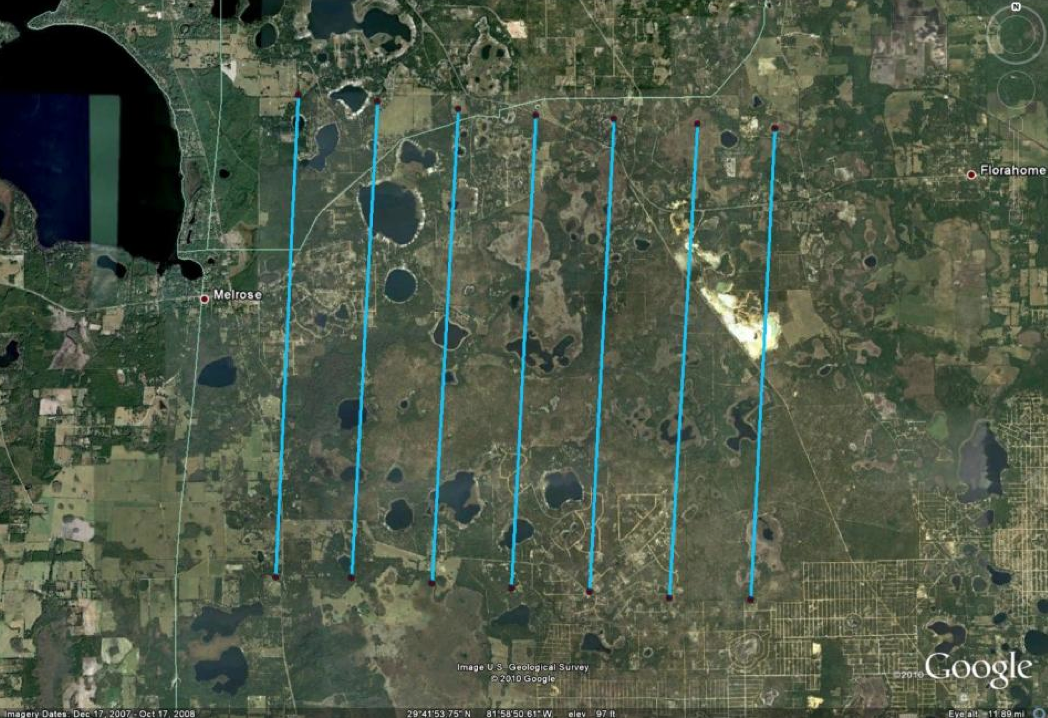
\includegraphics[height=1.7in,keepaspectratio]{./images/JPL_AVIRIS_flight_ground_tracks_OSBS_9_4_10.png}}\hspace{1em}%
  \subcaptionbox{Hyperspectral true-color mosaic, morning 09/04/2010\label{fig3:gaussian smoothing:a}}{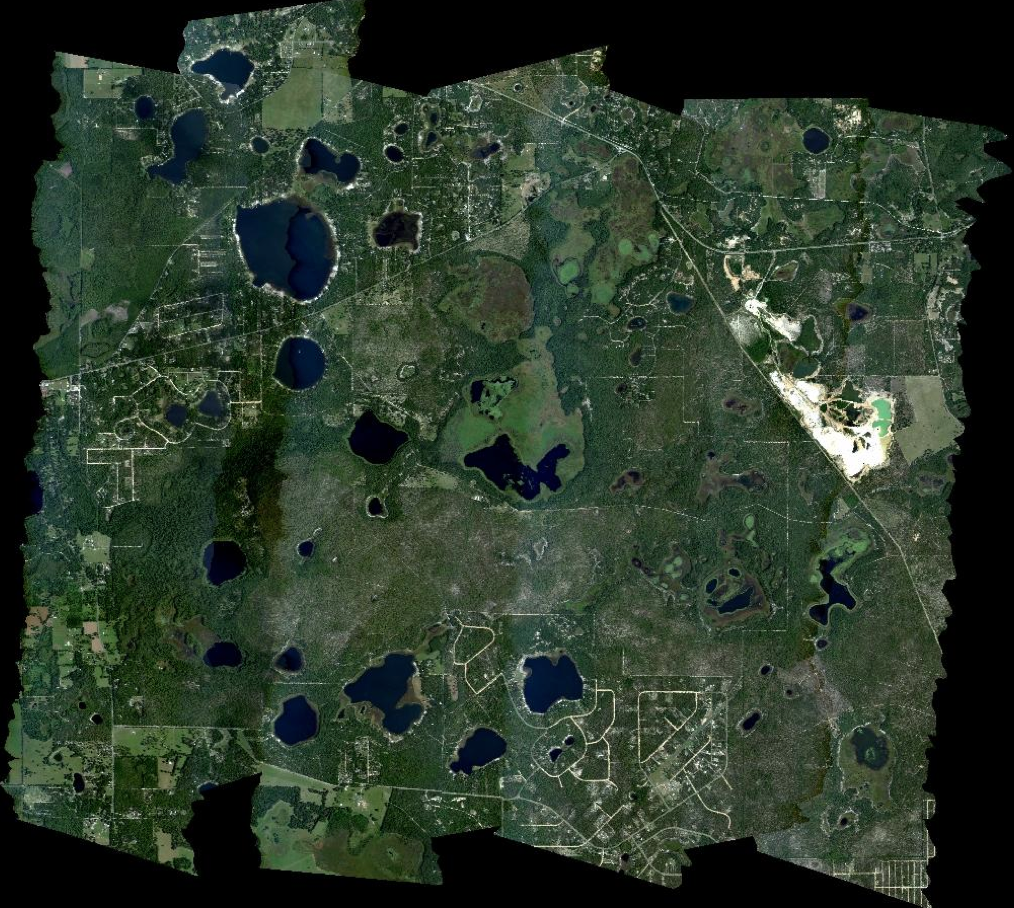
\includegraphics[height=1.7in,keepaspectratio]{./images/JPL_AVIRIS_true_color_mosaic_OSBS_9_4_10.png}}\hspace{1em}%
  \subcaptionbox{Hyperspectral true-color mosaic, mid-day 09/10/2010\label{fig3:gaussian smoothing:b}}{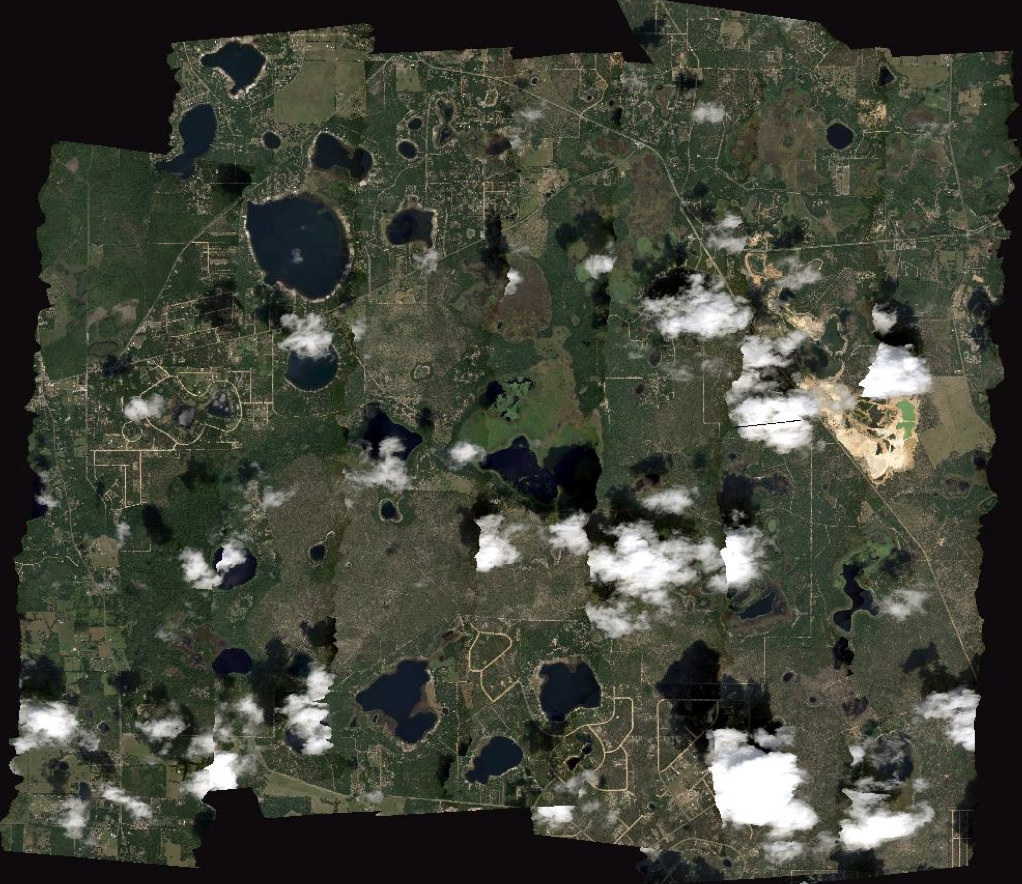
\includegraphics[height=1.7in,keepaspectratio]{./images/JPL_AVIRIS_true_color_mosaic_OSBS_9_10_10.png}}
   \caption{JPL AVIRIS flights over OSBS \cite{neon2010aopdatarelease}}
 \label{fig:hyperspectral}
\end{figure}



\textbf{Hypercpectral}: 
AVIRIS (Airborne Visible/Infrared Imaging Spectrometer) operated by personnel from the Jet Propulsion Laboratory (JPL) deployed on a Twin Otter DeHavilland DHC-6-300 aircraft in partnership with the National Aeronautics and Space Administration Terrestrial Ecology Program was used to collect data. 
JPL has flown on two separate days over OSBS: morning of September 4, 2010 (between 9:30 and 10:30 am) and mid-day of September 10, 2010. 
Both of the flights were flown at approximately $4000m$ AGL at approximately $90$ knots with zenith angle of $180.0$ and azimuth angle of $0.0$ with Altitude of $13kft$ (SOG ~ $65-91kts$)\footnote{NASA JPL AVIRIS Flight f100904t01: http://aviris.jpl.nasa.gov/cgi/flights\_10.cgi?step=view\_flightlog\&flight\_id=f100904t01 and http://aviris.jpl.nasa.gov/cgi/flights\_10.cgi?step=view\_flightlog\&flight\_id=f100910t01} at mostly clear with some haze for Sept. 4th and some puffies for Sept. 10th. 
Details of these flights can be seen in Figure \ref{fig:hyperspectral}. 
Dependent on flight line, pixel size ranges from $3.3m$ to $3.6m$. 
Hyperspectral data was atmospherically corrected using FLAASH \cite{adler1998flaash} and ATCOR \cite{richter2005atmospheric} algorithms. 
There are eight flight lines and the total size of which is 20.5GB for FLAASH and 10.2GB for ATCOR data. 
There are 224 bands recorded with wavelengths from $365.93 nm$ to $2496.24 nm$. 
%Concurrent ground data includes weather parameters, aerosol optical depth, field spectra of various canopies, and Leaf Area Index (LAI) measurements.

Atmospheric characterization relied on measurements of a CIMEL sun photometer in coordination with the NASA Aerosol Robotic Network\footnote{NASA AERONET: http://aeronet.gsfc.nasa.gov/cgi-bin/bamgomas\_interactive}. 
Measurements were collected on September 4, 2010 and the derived atmospheric information was used to improve the atmospheric correction of the AVIRIS spectrometer data. 
Detailed measurements such as aerosol optical thickness, water vapor, and etc are available online\footnote{OSBS Aero Measurements: http://aeronet.gsfc.nasa.gov/cgi-bin/type\_one\_station\_opera\_v2\_new?site=Ordway-Swisher}. 
FLAASH atmospheric correction is approximated as below \cite{adler1999atmospheric}:

\begin{equation}
L_e \approx (\frac{(A+B)\rho_e}{1-\rho_e S}+L_a)
\end{equation}

where $ \rho_e$ is an average surface reflectance for the pixel and a surrounding region, $S$ is the spherical albedo of the atmosphere, $L_a$ is the radiance back scattered by the atmosphere, and $A$ and $B$ are coefficients that depend on atmospheric and geometric conditions but not on the surface. 
On the other hand, ATCOR performs atmorpheric correction as follows \cite{Richter2014atcor}:

\begin{equation}
\rho =\frac{\pi \{ d^2 (c_0 + c_1 D N) - L_{path}\}}{\tau E_g}
\end{equation}

where $\tau$ is the atmospheric (direct or beam) transmittance for a vertical path through the atmosphere, $d$ is the earth-sun distance in astronomical units, $c_0$, $c_1$ and $ D N$ are the radiometric calibration offset, gain, and digital number, respectively. 
$\rho$ is the surface reflectance and $E_g$ is the global flux on the ground. 

%You can find various measured atmospheric parameters on the OSBS Aero Measurements website.

\textbf{LiDAR}: The National Center for Airborne Laser Mapping (NCALM)\footnote{http://www.ncalm.cive.uh.edu/} coordinated the waveform-LiDAR flights in the same study areas and as  with the AVIRIS flights as displayed in Figure \ref{fig:lidar} \cite{neon2010aopdatarelease}. 
NCALM flew an Optech Gemini\footnote{Optech Gemini LiDAR sensor: http://www.optech.ca/gemini.htm} waveform-LiDAR with a nominal altitude flight covering the entire OSBS on September 1, 2010. 
In total there were 33 flight lines collected over OSBS both in the morning and in the afternoon, 7 flight lines were re-flown due to clouds. Range scale of LiDAR data was at $1.0 m$ and up to five returns were recorded. 
The parameters for the data collected are $70 kHz PRF$, wide beam divergence of $0.8 mrad$, $20 deg$ half scan angle, and $40 Hz$ scan frequency. 
The GPS/IMU navigation data are processed using the Applanix POSPac MMS software to determine the position, orientation, and trajectory of the aircraft. 
The discrete LiDAR return data are processed using the Optech DASHMap software to create point cloud data files in ASPRS LAS 1.2 format \cite{las12format}. 
Each point data record contains information such as the intensity for the laser pulse and the X, Y, and Z geolocation of the point return. 
DASHMap reports up to four discrete returns: first, second, third, last. 
Using the geolocation information, the point clouds can be visualized 3-dimensionally.

% http://tex.stackexchange.com/questions/42968/reduction-of-space-between-two-sub-figures
\begin{figure}[tp]
  % Fixed length
  \centering
  \subcaptionbox{Flights ground tracks\label{fig3:gaussian smoothing:a}}{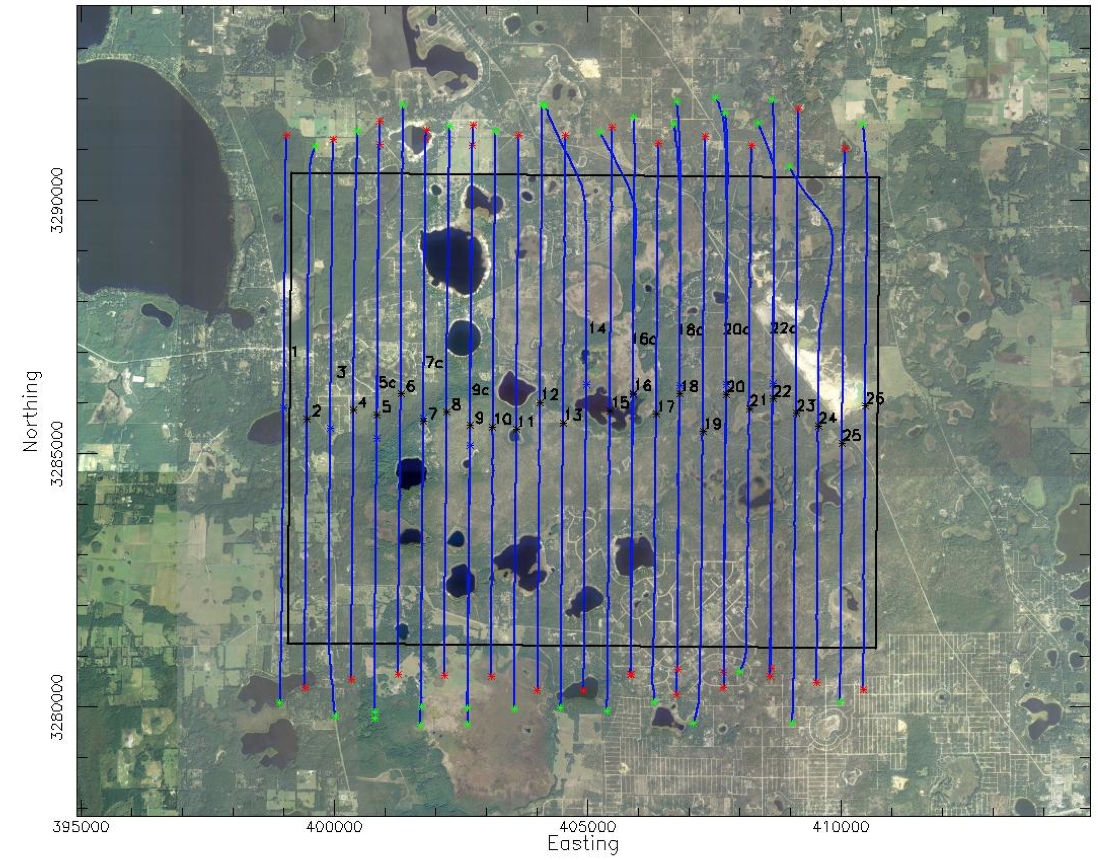
\includegraphics[height=2.3in,keepaspectratio]{./images/NCALM_flight_ground_tracks_OSBS_9_01_10.png}}\hspace{3em}%
  \subcaptionbox{LiDAR color height mosaic\label{fig3:gaussian smoothing:b}}{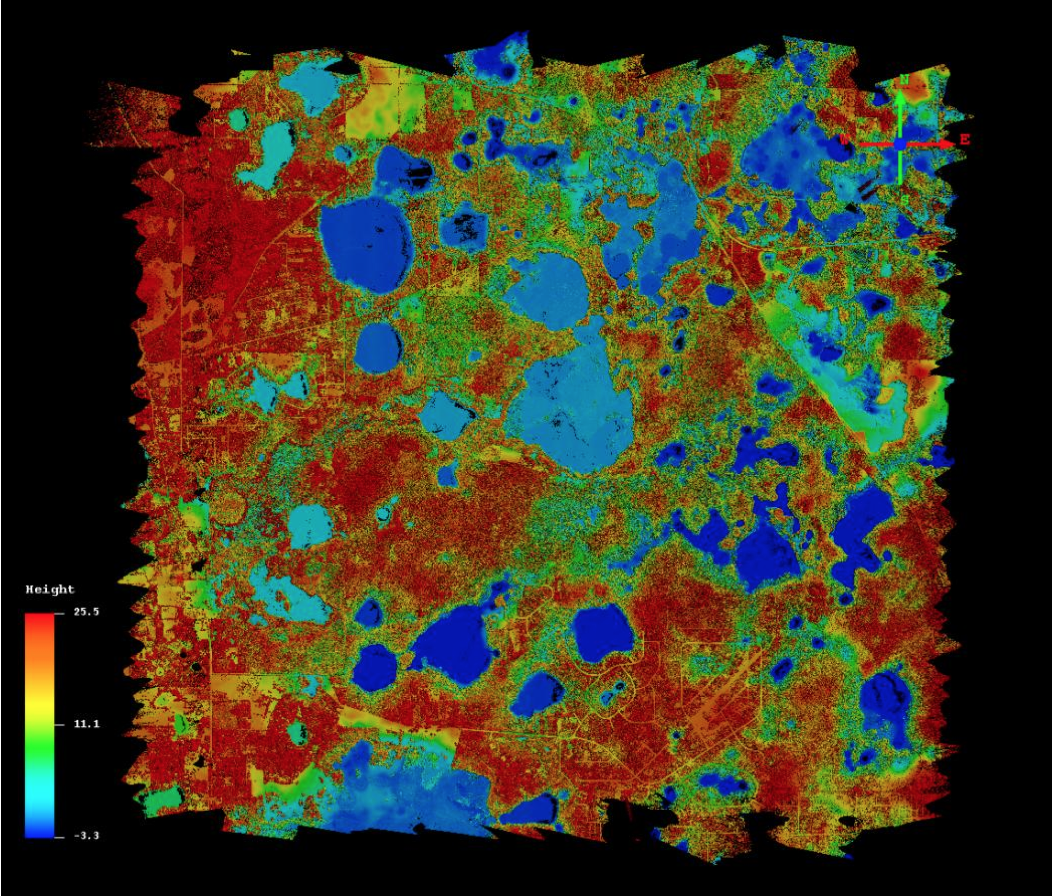
\includegraphics[height=2.3in,keepaspectratio]{./images/NCALM_Optech_Gemini_LiDAR_color_height_mosaic_OSBS_9_01_10.png}}
   \caption{NCALM Optech Gemini LiDAR flights over OSBS 09/01/2010 \cite{neon2010aopdatarelease}}
 \label{fig:lidar}
\end{figure}



\section{species Classification}

Upon the collection, orthorectification and atmospheric correction of hyperspectral and LiDAR data we work on identifying tree species. 
With the resolution of images being about 3 meters we are not getting pure pine or oak signals and there is lots of mixing pixels. 
A pixel's hyperspectral values can be a linear/nonlinear mixing of leaf, branch, soil, shade, and other signals. 
The timing of fights (September) adds to the challenge: leafs might not be as green or some trees might have already started to lose leaves and this leads to us getting more branch signals. 
Furthermore Longleaf Pine is a conifer (needlelaf), unlike broadleaf trees where signal return can be more accurate. 

\subsection{Field Data}


For our classification task, we collected ground data of identifying tree species on February 28th, 2014. 
We drove to OSBS with a laptop that has ArcMap installed on and the ENVI image loaded on, we connected a professional grade GPS to the laptop. 
ArcMap reads GPS coordinates and mapped the polygons in the ENVI image. 
In this way, we marked several geo-polygons that had similar plant species in the ENVI image. 
Later on we overlayed the identified polygons with proper JPL AVIRIS flight which had the least amount of clouds. 
This approach works pretty accurate if you are not in a dense forest such as tropical forests where GPS signal under the tree canopy has high deviations due to NLOS (no-line of sight) of GPS signals. 
Even with these considerations, commercial GPS have sub-meter accuracy and when combined with error accumulated in orthorectification of flight images we still need to mark several land marks such as roads, big trees and etc to be able to re-verify marked points in the map and avoid shifts in coordinates.

Altogether we identified species for 1269 pixels. In Table \ref{table:field data} you can find the details of identified Regions of Interest (ROIs) along with their details. 

\begin{table}[t]
\scalebox{0.65}{
\begin{tabular}{ccccccccccccc}
&\multicolumn{8}{ c }{Broad Leaf}&\multicolumn{4}{ c }{Conifer}\\
 \textbf{Specie} & \multicolumn{2}{c}{Oak (other)} & \multicolumn{2}{c}{Laurel Oak} & \multicolumn{2}{c}{Live Oak} & \multicolumn{2}{c||}{Turkey Oak} & \multicolumn{2}{c}{Pine  (other)} & \multicolumn{2}{c}{Longleaf Pine} \\ 
 & ROI Id & \# of Pixels              & ROI Id & \# of Pixels         & ROI Id & \# of Pixels         & ROI Id & \multicolumn{1}{c||}{\# of Pixels} & ROI Id &  \# of Pixels    & ROI Id & \# of Pixels \\ %\cline{2}
 & 23     & \multicolumn{1}{ c| }{62} & 52 &\multicolumn{1}{ c| }{29} & 4  &\multicolumn{1}{ c| }{48} & 10 & \multicolumn{1}{ c|| }{73}& 20        & \multicolumn{1}{ c| }{68} &  12    &107\\
 & 19     & \multicolumn{1}{ c| }{19} & 50 &\multicolumn{1}{ c| }{20} & 13 &\multicolumn{1}{ c| }{37} & 15 & \multicolumn{1}{ c|| }{34}& 14        & \multicolumn{1}{ c| }{67} &  9     &30\\ 
 & 17     & \multicolumn{1}{ c| }{15} & 49 &\multicolumn{1}{ c| }{17} & 28 &\multicolumn{1}{ c| }{22} & 21 & \multicolumn{1}{ c|| }{33}& 2         & \multicolumn{1}{ c| }{30} &  45    &23\\
 & 35     & \multicolumn{1}{ c| }{15} & 48 &\multicolumn{1}{ c| }{9 } & 29 &\multicolumn{1}{ c| }{22} & 11 & \multicolumn{1}{ c|| }{26}& 5         & \multicolumn{1}{ c| }{24} &  18    &22\\
 & 36     & \multicolumn{1}{ c| }{10} & 53 &\multicolumn{1}{ c| }{6 } & 30 &\multicolumn{1}{ c| }{22} & 6  & \multicolumn{1}{ c|| }{23}& 3         & \multicolumn{1}{ c| }{20} &  44    &21\\
 &        &                           &    &                          &    &                          & 34 & \multicolumn{1}{ c|| }{23}& 42        & \multicolumn{1}{ c| }{17} &  37    &17\\
 &        &                           &    &                          &    &                          & 31 & \multicolumn{1}{ c|| }{18}& 43        & \multicolumn{1}{ c| }{16} &  16    &16\\
 &        &                           &    &                          &    &                          & 25 & \multicolumn{1}{ c|| }{17}& 1         & \multicolumn{1}{ c| }{13} &  40    &15\\
 &        &                           &    &                          &    &                          & 26 & \multicolumn{1}{ c|| }{16}& 22        & \multicolumn{1}{ c| }{10} &  47    &14\\
 &        &                           &    &                          &    &                          & 32 & \multicolumn{1}{ c|| }{16}& 38        & \multicolumn{1}{ c| }{10} &  39    &12\\
 &        &                           &    &                          &    &                          & 27 & \multicolumn{1}{ c|| }{15}&           &                           &  41    &12\\
 &        &                           &    &                          &    &                          & 7  & \multicolumn{1}{ c|| }{14}&           &                           &  46    &11\\
 &        &                           &    &                          &    &                          & 24 & \multicolumn{1}{ c|| }{13}&           &                           &  8     &7 \\
 &        &                           &    &                          &    &                          & 33 & \multicolumn{1}{ c|| }{13}&           &                           &        &  \\
\textbf{Total} & 5 ROIs & 121 Pixels & 5 ROIs & 81 Pixels & 5 ROIs & 151 Pixels & 14 ROIs & \multicolumn{1}{ c|| }{ 334 Pixels } & 10 ROIs & 275 Pixels& 13 ROIs& 307 Pixels\\%\cline{2-9}\cline{11-12}
\textbf{Partial Total} &\multicolumn{8}{ c|| }{29 ROIs - 687 Pixels}&\multicolumn{4}{ c }{23 ROIs - 582 Pixels}\\ \hline
\textbf{Grand Total} & \multicolumn{12}{c}{52 ROIs - 1269 Pixels}     
\end{tabular}
}
	
\caption{Field Data Specifications}
\label{table:field data}

\end{table}

% http://tex.stackexchange.com/questions/42968/reduction-of-space-between-two-sub-figures
\begin{figure}[tp]
  % Fixed length
  \centering
  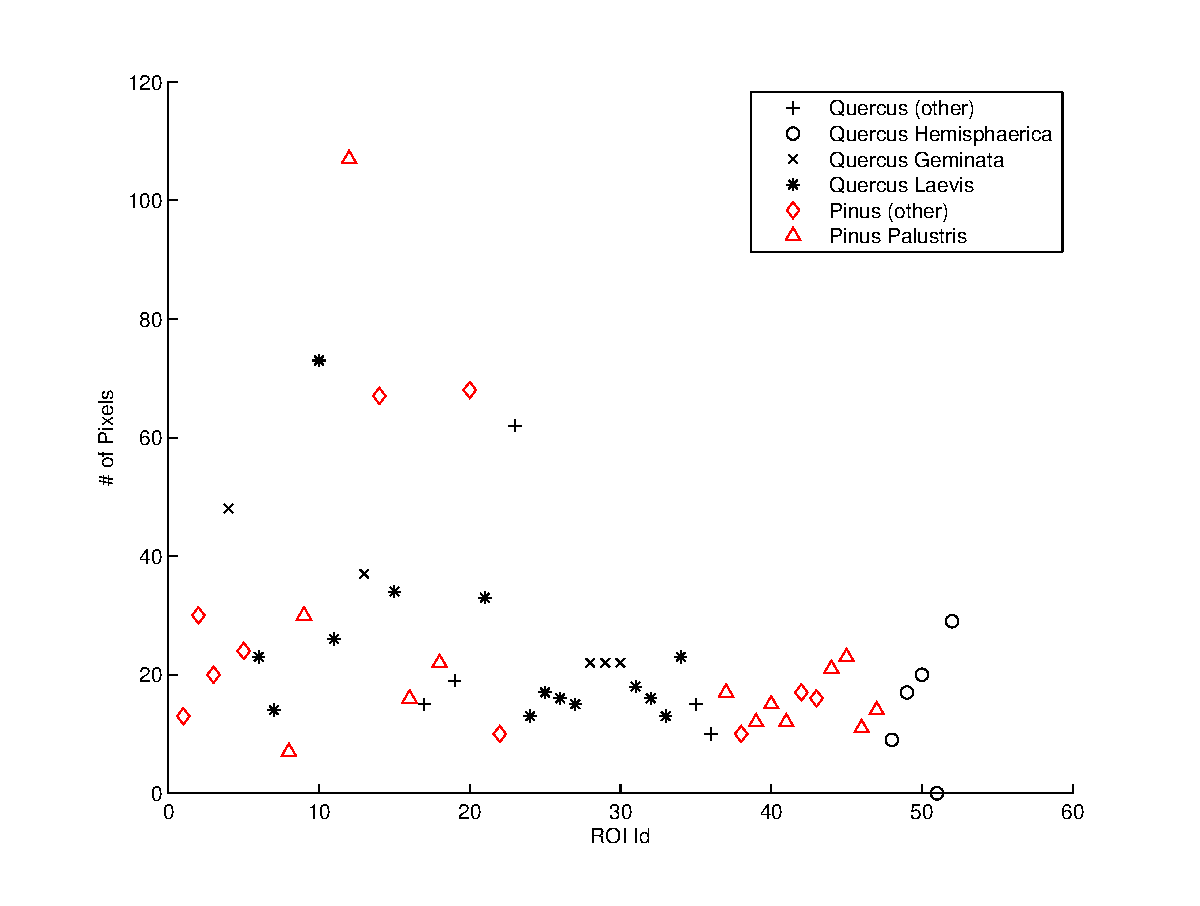
\includegraphics[height=3in,keepaspectratio]{./images/fieldData.eps}%
   \caption{Field Data Distribution of ROIs}
 \label{fig:lidar}
\end{figure}


The closer ROI Ids are means that they are collected at a closer vicinity (geographically/temporally), and the more distant ROI ids means that canopies are more apart. 
You can see that some species have lots of abundance (334 for Turkey Oak) and some have few (81 for Laurel Oak) this bias in population size inadverently affect classification accuracy.

The Oak  (other) species represent generic oak specie (\textit{specie details unknown}). Live Oak is specifically Sand Live Oak (\textit{Quercus Geminata}), Laurel Oak represents \textit{Quercus Hemisphaerica}, Turkey Oak is \textit{Quercus Laevis}, Longleaf Pine is \textit{Pinus Palustris}, and Pine (other) represents a mixture of different varieties of pines:  Longleaf Pine (\textit{Pinus palustris}), Loblolly Pine(\textit{Pinus Taeda}) or Slash Pine (\textit{Pinus Elliottii}).

We use a combination of grid search and heuristics to adjust SVM parameters for better performance.

\subsection{Preprocessing}

We load hyperspectral images in Matlab using an in-house upgraded version of \texttt{enviread}, initially developed by Dr. Ian Howat at Ohio State University \cite{howat2007enviread}. 
We check for the consistency of calibration and uniformness of pixel sizes. 
As different flights have different altitudes and hence pixel resolutions, this is an essential step to account for. 
Defining a hyperspectral image $I$ with dimensionality $(x,y,w,z)$, where $x \in X = [167000, 833000 ]$ meters represents the range of UTM Easting values, $y \in Y = [0, 9400000]$ meters represents UTM Northing values, $w \in W = \{1, \dotsc, 224\}$ is the index of the reflectance wavelengths, and $z \in Z = \{1, \dotsc, 60 \}$ is the UTM zone of the image. 
Based on our observations, we take constant $\xi = 10000$ as a cut-off point to avoid erroneous sensor readings. 
There are some noises in JPL AVIRIS measurements such as negative reflectance values; 
the range of hyperspectral reflectance values is in range $[-32762, 32724]$: one should note that reflectance is the proportion of sun radiance signals which should be a positive value, but in normalized form reflectance is between zero and one. Below you can see the normalization process:

\begin{equation}
I_{xywz} = \left\{ \begin{array}{rcl}
0 & \mbox{for} & I_{xywz} < 0 \\ 
1 & \mbox{for} & I_{xywz} > \xi \\
\sqrt{\frac{I_{xywz}}{\xi}} & \mbox{otherwise} & 
\end{array}\right.
\end{equation}

To normalize we set negative reflectance values to zero and values greater than 10,000 to 10,000. 
To enhance the intensity of readings we take the square-root of signal returns. 
This procedure is due to the following facts: 
a) There is no standard output of reflectance data and even reflectance of a single crown at different pixels can be quiet different.
 Unlike minerals that have fixed and known reflectance values, trees can different signal returns based on generation, condition of growth (water quality, climate, soil, and etc) which can make this task challenging. 
 b) We do not have ground reflectance values produced by NEON available to us. 
 c) Due to low resolution of images signals are all mixed. 
 Due to these reasons, empirically obtained thresholds and ranges are inevitable. 
 Regarding square root, one should note that without taking the square root the images lack proper day-light intensity and appear dark.

\subsubsection{Filter Water Absorption Bands}

In our calculations wavelengths corresponding to strong water vapor absorption bands in the atmosphere are excluded. 
This includes 1333.2$nm$ to 1482.7$nm$, 1791.6$n m$ to 1967.4$n m$, and 2406.9$n m$ to 2496.2$n m$. 
Due to strong absorption at those wavelengths, a small radiance signal is measured by the instrument. 
This leads to errors in the reflectance calculation (as several highly random upward spikes in reflectance plots). 

\subsubsection{Filter Non-vegetated/Shaded Pixels}

A filter of $NIR < 0.33$  excludes heavily shaded samples  which usually have distorted reflectance signals \cite{colgan2012mapping}. 
Normalized Difference Vegetation Index (NDVI) is an index which shows how green a pixel is and is usually used to remove material that does not belong to planetary material such as roads, clouds and any not-vegetated area, even grass and so on. By properly applying an NDVI filter you will end up in major tree crowns.
As you can see in \ref{table:field data}, we have tens of pixels per ROI and considering that each pixel is about $3m$ wide and the fact that the species look into do not have wide crowns; this means that ROIs are generously marked and span several tree crowns. 
This includes the empty spaces between crowns, some shady pixels, understory grass, and etc. 
From within such generous canopy the initial belief is that to properly classify tree species we should get rid of low NDVI pixels from such large canopies. 
Contrary to this belief due to the mixing nature of hyperspectral pixels and aggregate operation of classificaion techniques in multi-dimensional space, removing low NDVI pixels from tree canopies degraded classification performance by about 10\%. The take away of this experiment was that for specifically marked canopies it is better to preserve even low NDVI pixel as they might have some added value in the aggregate operation of the classification algorithm.
NDVI is defined as below:

\begin{equation}\label{xx}
NDVI  = \frac{NIR - VIS}{NIR + VIS}
\end{equation}

where is $NIR$ the reflectance in the reflective near-infrared wavelengths (725-1100 $n m$) and $VIS$ is the reflectance in the visible (red) wavelengths (580-680 $n m$). 
The principle behind this is that $VIS$ is in a part of the spectrum where chlorophyll causes considerable absorption of incoming radiation, and the $NIR$ is in a spectral region where spongy mesophyll leaf structure leads to considerable reflectance \cite{tucker1979red, jackson1983discrimination}. 
For this purpose we chose the band at 665.6 $n m$ for red and 734.1 $n m$ for near-infrared. 
By filtering out pixels with $NDVI < 0.4$ we are essentially removing pixels that are not green. 

\subsubsection{Gaussian Filter}

Real-life sensor measurements are far from perfect and there are many nosy readings along different bands. 
We take advantage of abundance of bands (224 bands) and take use of their aggregated information by applying a Gaussian filter. 
We take a Gaussian window $w$ of size $N > 0$, the coefficients of a Gaussian window are computed as below:

\begin{equation}
w(n) = e^{-\frac{1}{2}(\alpha \frac{n}{N/2})^2}
\end{equation}  

where $-\frac{(N-1)}{2} \leq n \leq \frac{(N-1)}{2}$, and $\alpha$ is inversely proportional to the standard deviation ($\sigma$) of a Gaussian random variable ($\sigma = \frac{N}{2\alpha}$). 
Once we have Gaussian parameters we perform convolution to apply the smoothing factor. 
By convolving vectors $u \in \mathbb{R}^m$ and $v\in \mathbb{R}^n$, we will have vector $w\in \mathbb{R}^{m+n-1}$ such that: 

\begin{equation}
w(k)=\sum_j u(j)v(k-j+1)
\end{equation} 


\subsection{Support Vector Machines}

It is well known in literature that Support Vector Machines (SVM) outperforms other algorithms on species classification \cite{colgan2012mapping, baldeck2014landscape, cho2012mapping}. 
Our focus is on the impact of atmospheric corrections (FLAASH vs ATCOR) at pixel level classification using \textit{non-linear multi-class SVM}. 
We parametrize SVM with $k$-fold cross validation where $k=5$, which means for each model we perform classification 5 times where at each time a separate non-overlapping portion of ground data is specified for train and test purposes. 
The ratio of train vs test is 4 to 1 from total samples.
We 


Classifier non-linearity comes from taking the following non-linear functions as kernel for SVM: 

\begin{itemize}
\item Polynomial function kernel.
\item Radial Basis Function (RBF) kernel
\end{itemize}

Regarding multi-class classification, we create $\binom{c}{2}$ classifiers where $c$ is the number of classes. 
In this case $c=6$, hence we train $\binom{6}{2} = 15$ classifiers at each iteration of $k$-fold.
We train all the classifiers and to decide on the class a given test case belongs to, we perform majority voting among classifiers to decide the class of each pixel. 
We avoid aggregating canopy pixels classes to determine the class of the canopy as this process can be performed using heuristics such as majority of pixels or etc, which is irrelevant to the purpose of pixel-level classification.
Furthermore, it might not be always feasible to assume that we always know the correct boundaries of a canopy in new data sets.







\section{Results and Discussion}

We study the impact of optimzing classifier parameters on FLAASH and ATCOR atmospheric corrections. 
Our focus is on the impact of data pre-processing filters on the performance of the species classificaion while we compare the two. 
An implementation of a one-vs-one multi-class k-fold cross-validation setup of SVM using non-linear kernels (polynomial and radial basis) functions is used for our model. 
In our scenario $k=5$ as for some of our species we only have 5 canopies and we canot $k>5$ for a valid implementation of k-fold cross validation.
Majority vote determines the specie of a pixel. 
Test and train sets are canopy-aware, meaning that pixels of a single canopy is either used for training or test sets and not both.
A mixture of grid search and heuristic optimization determines various parameters for SVM kernels, but for brevity we only present 2D diagrams here as other parameters settings are out of scope of this project. 
Specifically we set a cost of $C = \infty$ for misclassification, meaning that we have little to zero tolerance for improperly classified samples.



% http://tex.stackexchange.com/questions/42968/reduction-of-space-between-two-sub-figures
%\begin{figure}[tp]
%  % Fixed length
%  \centering
%  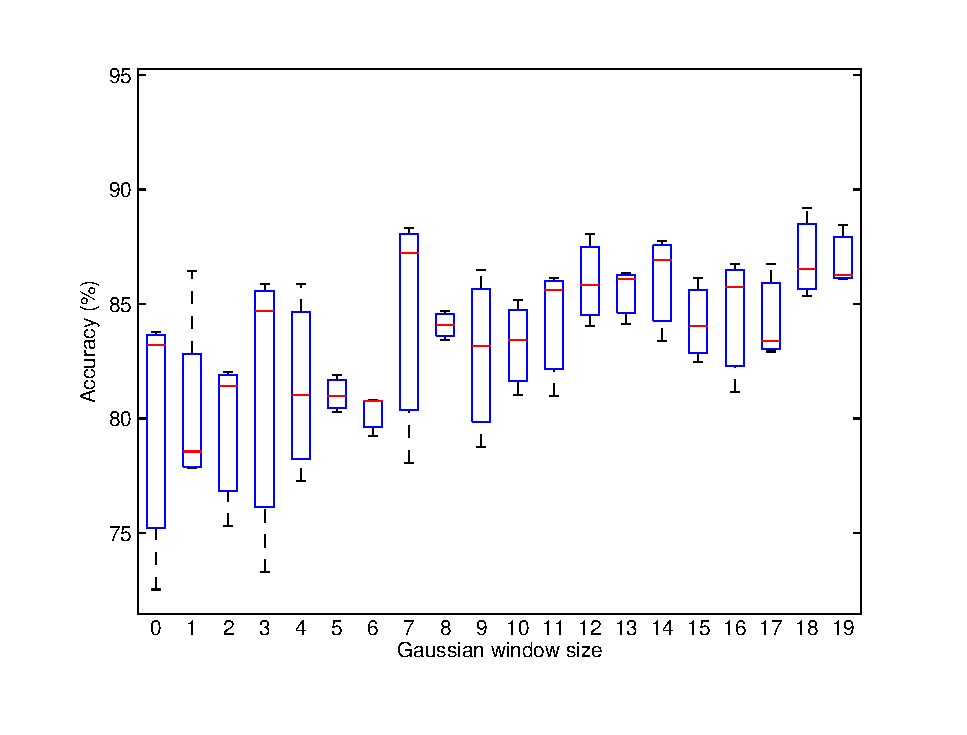
\includegraphics[height=3in,keepaspectratio]{./images/gaussian_window.eps}%
%   \caption{Impact of Gaussian Window on Prediction Accuracy}
% \label{fig:lidar}
%\end{figure}



% http://tex.stackexchange.com/questions/42968/reduction-of-space-between-two-sub-figures
%\begin{figure}[tp]
  % Fixed length
%  \centering
%    \subcaptionbox{After removing low NDVI NIR pixels\label{fig:after removing NDVI NIR}}{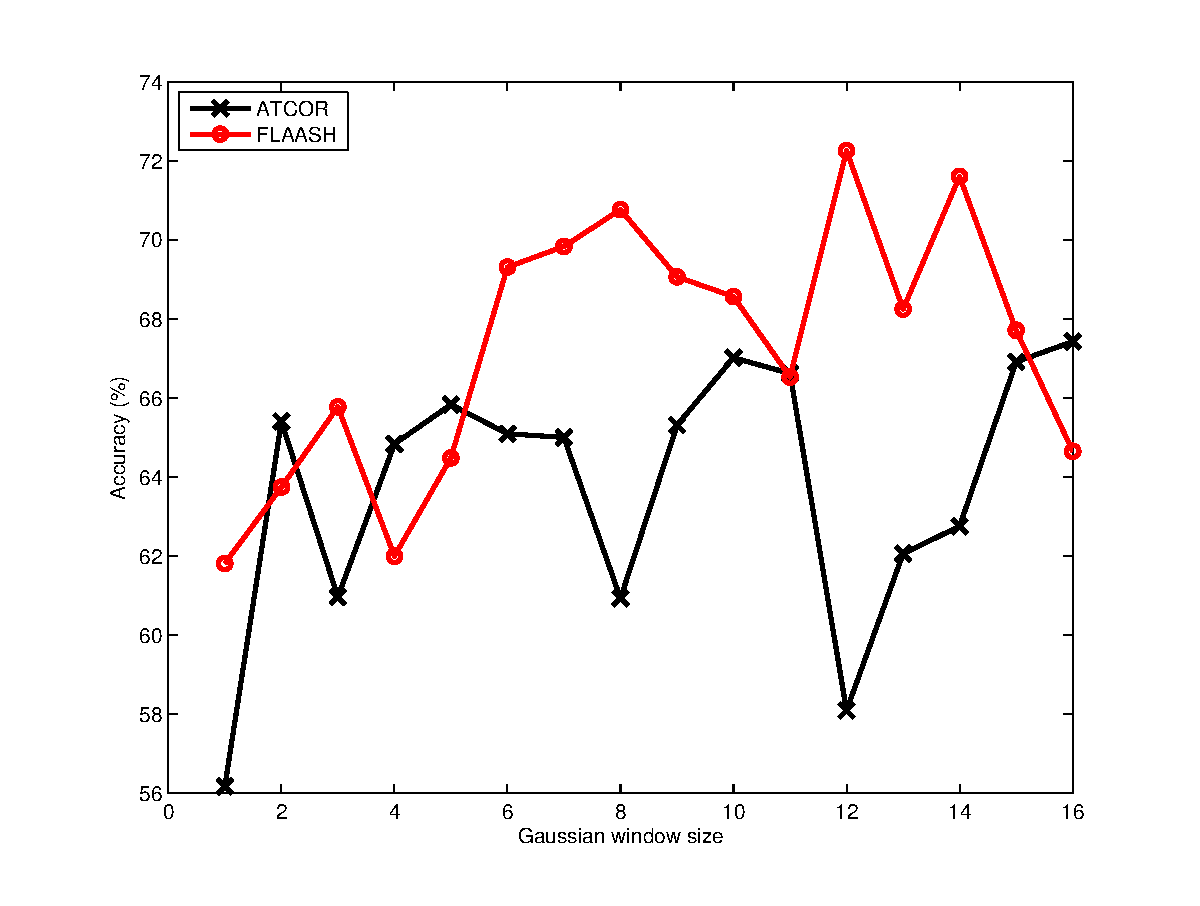
\includegraphics[height=2.5in,keepaspectratio]{./images/after-removing-ndvi-nir.eps}}\hspace{1em}%
%    \subcaptionbox{Generic 2/3 vs 1/3 train and test sets. Asserting non-overfitting SVM model\label{fig:13 23}}{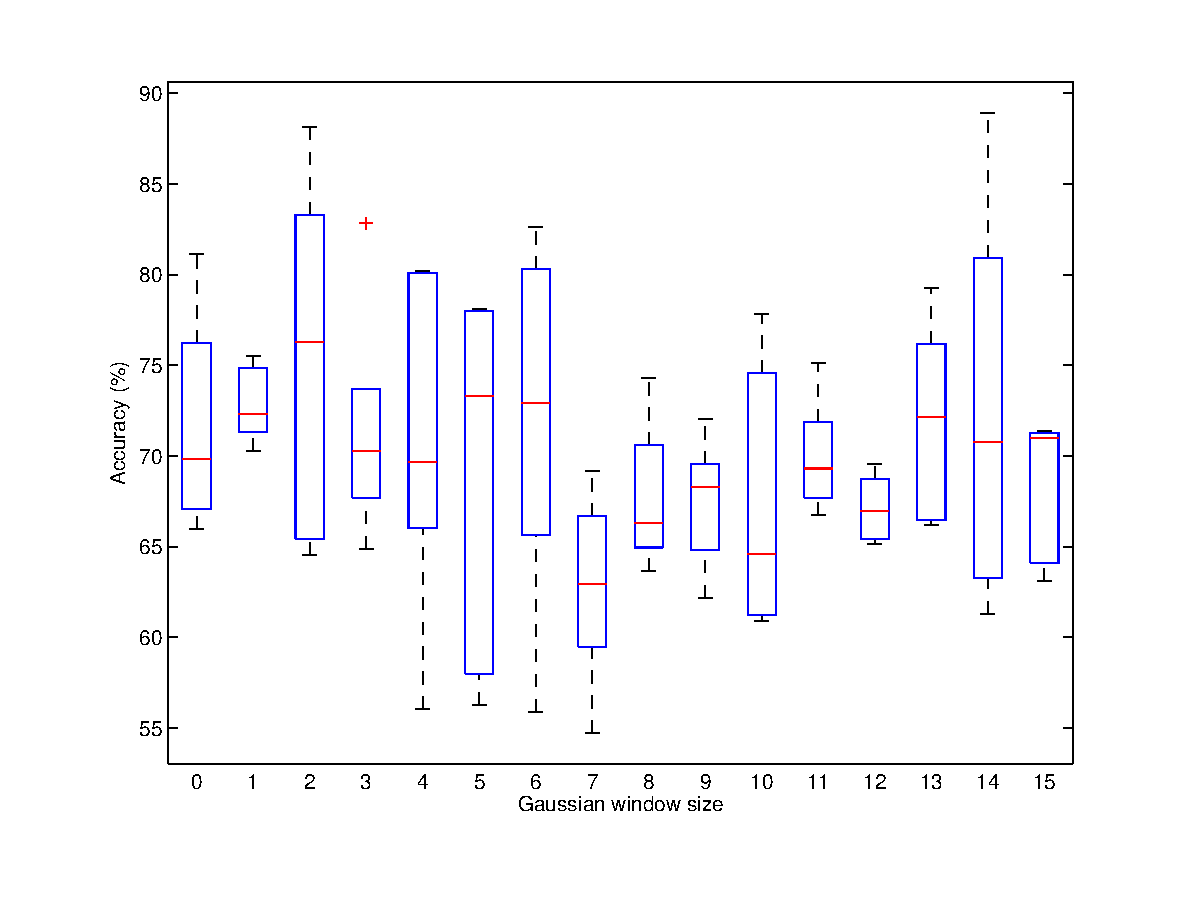
\includegraphics[height=2.5in,keepaspectratio]{./images/F-svm-13-23.eps}}\hspace{1em}%

%   \caption{Impact of Gaussian Window on Prediction Accuracy}
%       \label{fig:parameter tuning}
%\end{figure}

% water absorption bands
%ndvi nir
% gaussian
%poly rbf
%1/3 2/3
%conifer vs broadleaf (2 class)

% outlier detection via one class svm for future paper.

% http://tex.stackexchange.com/questions/42968/reduction-of-space-between-two-sub-figures
\begin{figure}[b!] %bthp
  % Fixed length
  \centering
  \subcaptionbox{Before removing water absorption bands\label{fig:before removing wab}}{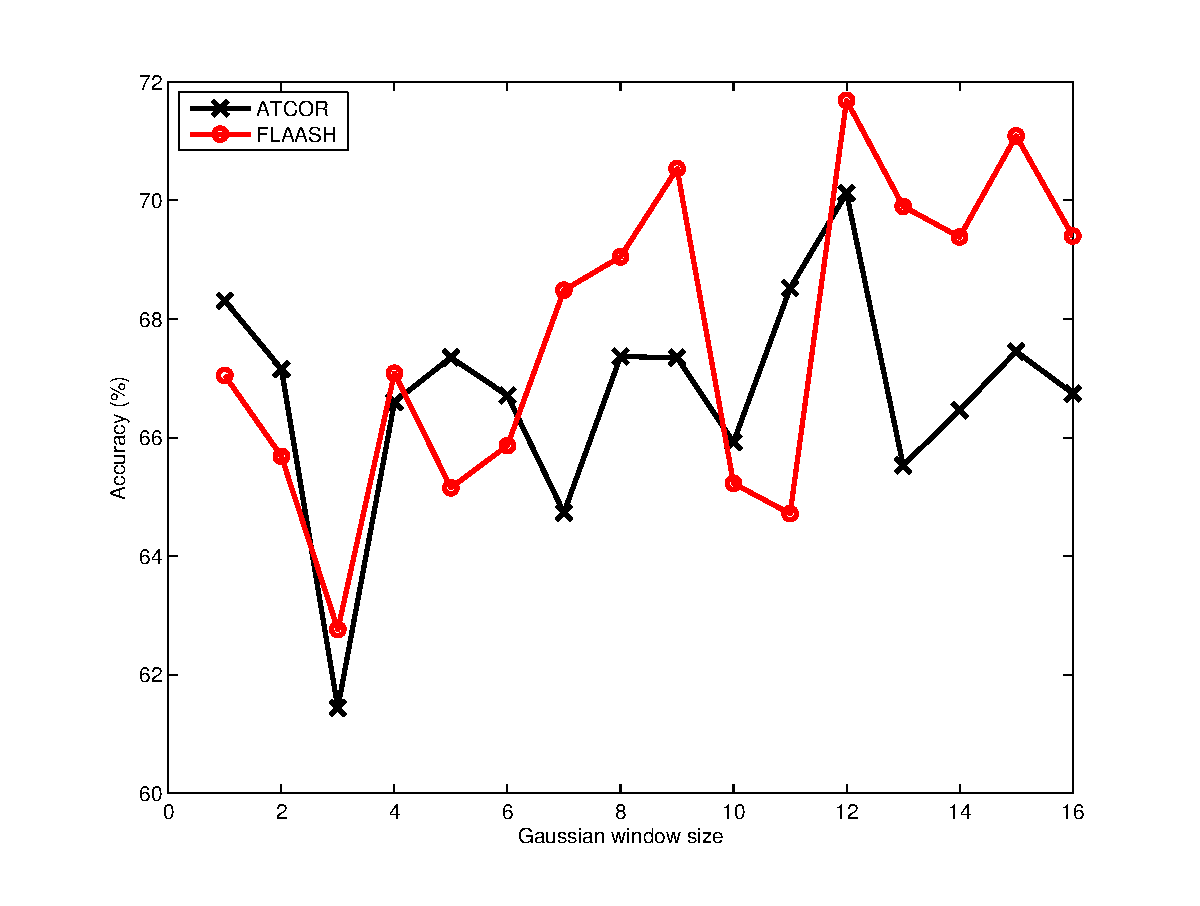
\includegraphics[height=2.5in,keepaspectratio]{./images/before-removing-wab.eps}}
  \subcaptionbox{After removing water absorption bands\label{fig:after removing wab}}{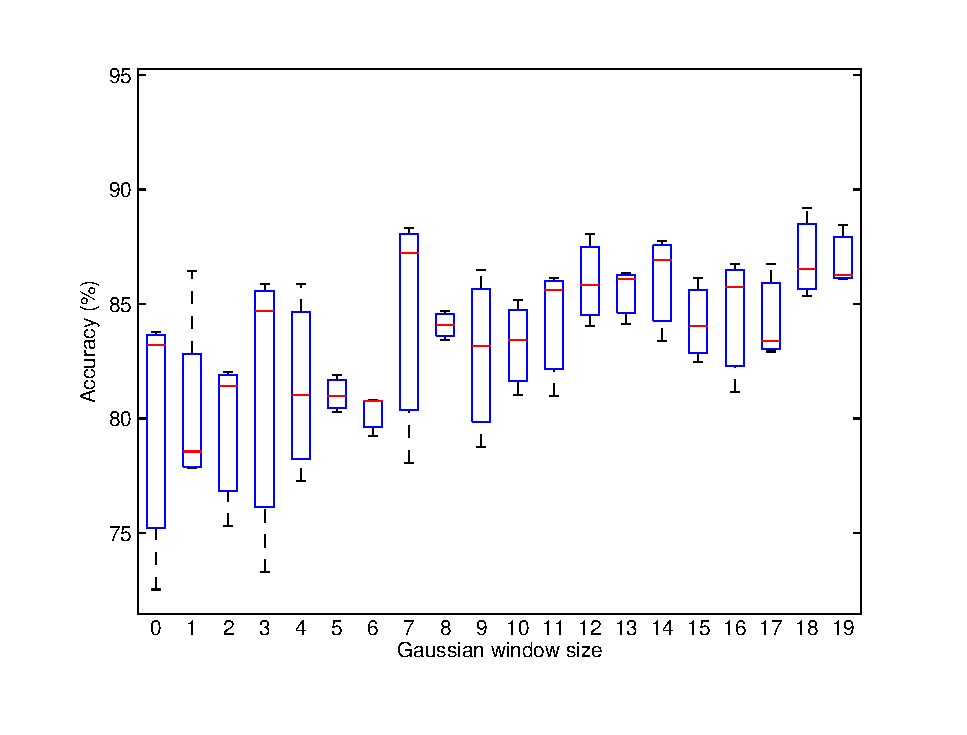
\includegraphics[height=2.5in,keepaspectratio]{./images/gaussian_window.eps}}\hspace{1em}%
   % \subcaptionbox{After removing low NDVI NIR pixels\label{fig:after removing NDVI NIR}}{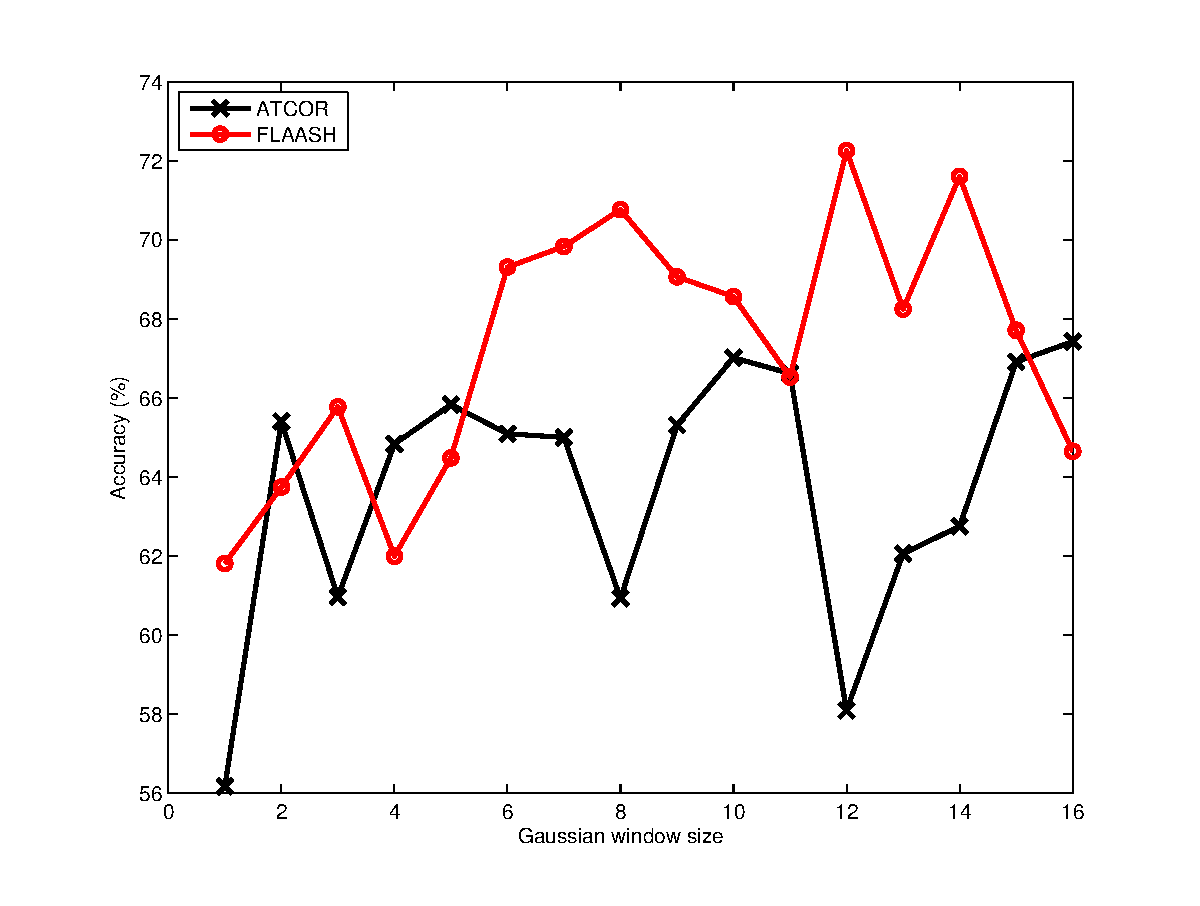
\includegraphics[height=2.5in,keepaspectratio]{./images/after-removing-ndvi-nir.eps}}\hspace{1em}%

   \caption{Impact of Gaussian Window on Prediction Accuracy}
       \label{fig:water absorption bands}
\end{figure}


In Figure \ref{fig:water absorption bands} we show how removing water absorption bands helps us improve prediction accuracy. 
Before removing these bands (Figure \ref{fig:before removing wab}) prediction accuracy starts at about 66\% and rises to about 71\% as we increase Gaussian window size (about 5\% performance improvement). 
There is a positive trend across different window sizes which means we can expect better accuracy the bigger the window size gets. 
This stems from the fact that water absorption bands add to randomness and as we increase window size this randomness is dissolved to the majority of neighbors and would have less and less impact as window size increases. 
After removing water absorption bands (Figure \ref{fig:after removing wab}) prediction accuracy starts at 74\% and rises to about 76.5\% at a window size of 8. 
Beyond that there is no significant change in accuracy.
%which is minimal change but on average you can see that applying a Gaussian filter increases accuracy by small margins (maximum 1\%). 
As window size increases you can see that there is no predictable impact of Gaussian smoothing in accuracy; 
This is due to the fact that all the currently available data signals has soem level of inherent entropy (less noisy) and increasing window size beyond certain point just takes data away from their original meaning which can either help or harm accuracy in unpredictable ways. 




% http://tex.stackexchange.com/questions/42968/reduction-of-space-between-two-sub-figures
%\begin{figure}[t]
%  % Fixed length
%  \centering
%  \subcaptionbox{Before removing water absorption bands\label{fig:before removing water absorbtion bands}}{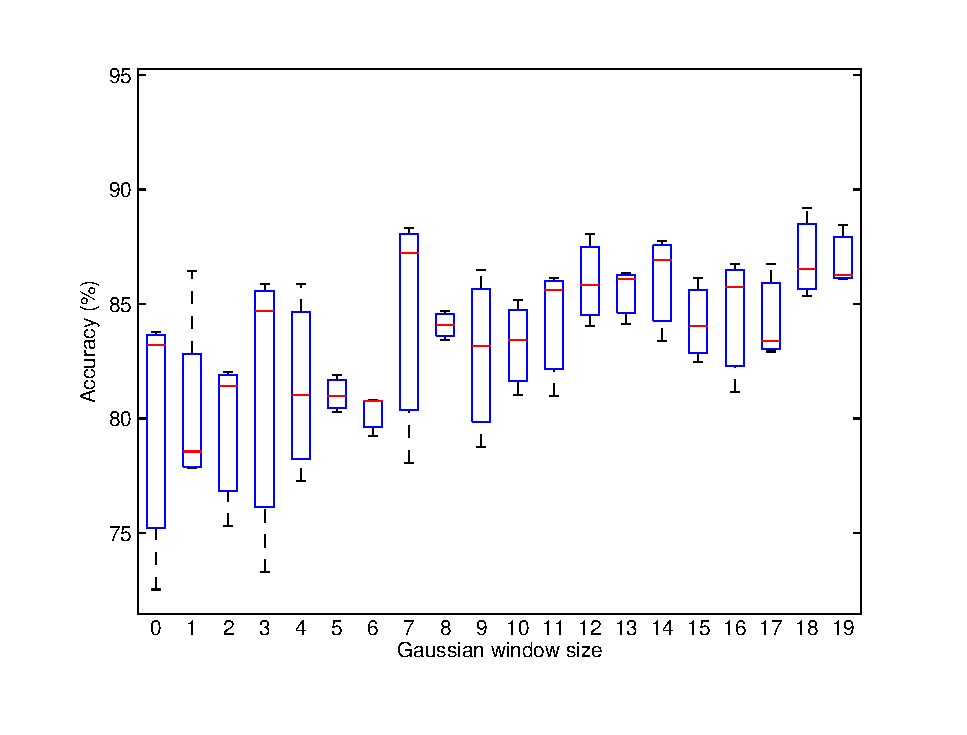
\includegraphics[height=2.3in,keepaspectratio]{./images/gaussian_window.eps}}\hspace{1em}%
%  \subcaptionbox{After removing water absorption bands\label{fig:after removing water absorbtion bands}}{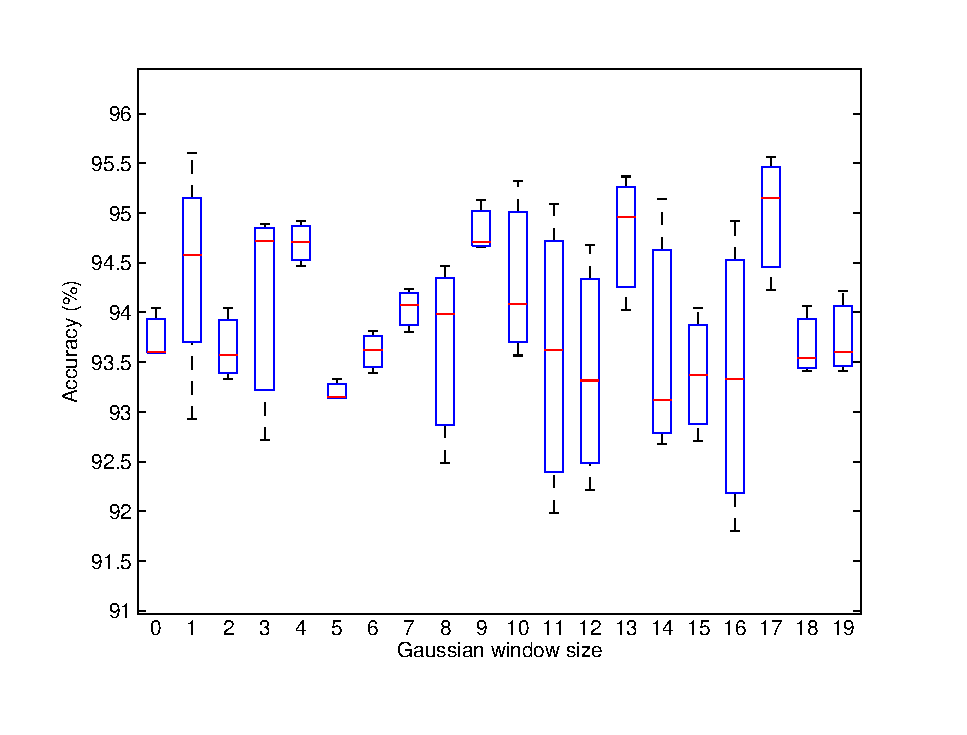
\includegraphics[height=2.3in,keepaspectratio]{./images/gaussian_window_filtered_water_absorbtion_bands.eps}}
%   \caption{Impact of preprocessing filters on classification accuracy using polynomial kernel degree 3 on ATCOR data before and after applying pre-processing filters}
% \label{fig:before-after removing water absorbtion bands}
%\end{figure}



% http://tex.stackexchange.com/questions/42968/reduction-of-space-between-two-sub-figures
%\begin{figure}[t]
  % Fixed length
%  \centering
%  \subcaptionbox{FLAASH atmospheric correction\label{fig:atmospheric correction:flaash}}{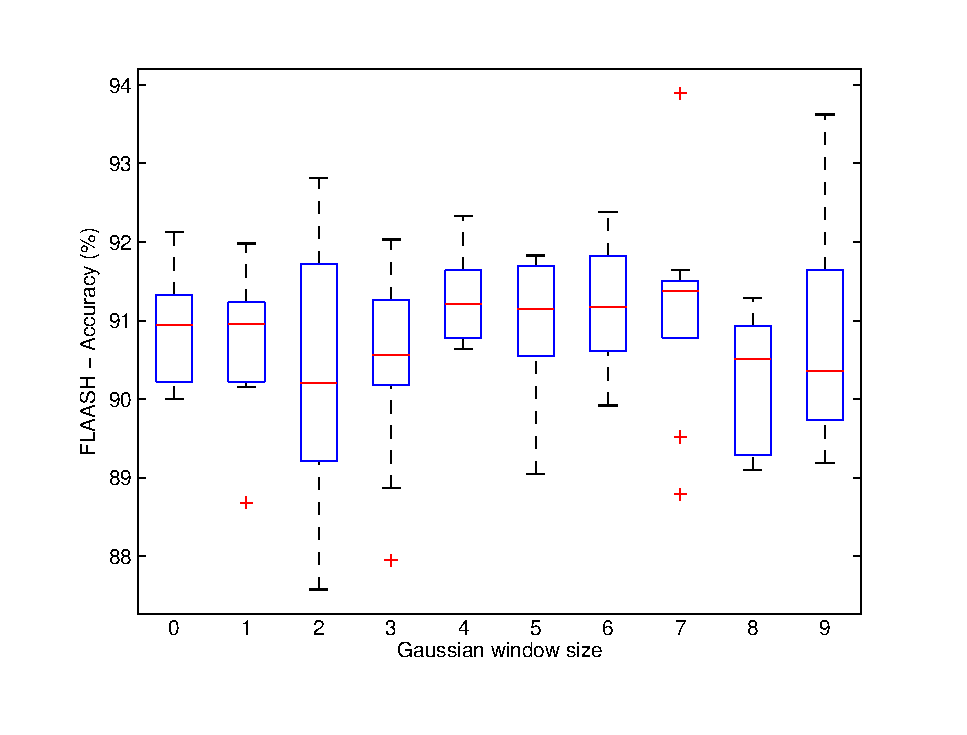
\includegraphics[height=2.3in,keepaspectratio]{./images/atcor_flaash/gaussian_flaash.eps}}\hspace{1em}%
%  \subcaptionbox{ATCOR atmospheric correction\label{fig:atmospheric correction:atcor}}{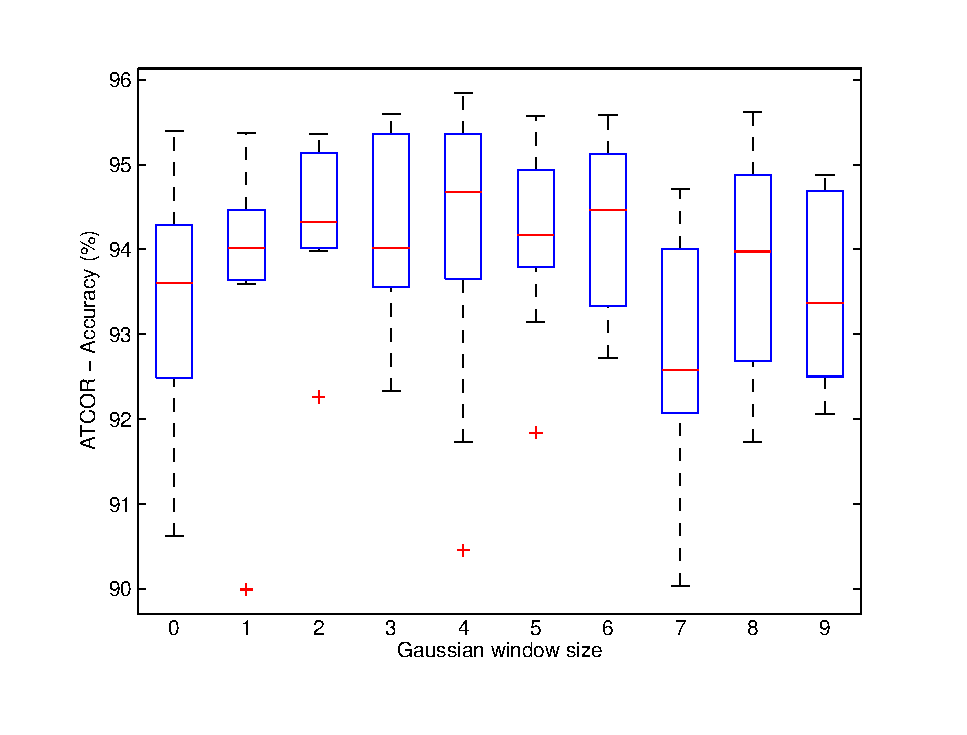
\includegraphics[height=2.3in,keepaspectratio]{./images/atcor_flaash/gaussian_atcor.eps}}
%   \caption{Impact of atmospheric correction on classification accuracy}
% \label{fig:atmospheric correction}
%\end{figure}

Next, we look at the impact of removing low NDVI-NIR pixels from dataset. As you can see in Figure \ref{fig:after removing NDVI NIR} there is a general degradation of performance from the previous scenairo that we used the whole dataset. 
In FLASSH dataset we are at about 70\% and ATCOR yields 66\% accuracy.
This is due to the fact that pixel size is large ($3m$) and canopies are large as well. 
According to Table \ref{table:field data}, canopy sizes are in the range of $[6,107]$ pixels. 
This generous marking of canopies includes areas with little green-ness, shaddows, branches and etc (low NDVI and low NIR values). 
But you should note that due to the mixing nature of reflectance values, even low NDVI/NIR pixels of a continous canopy still contains signals from the underlying species,
Which might not be as green.
Here we can see that including low NDVI/NIR pixels of a continous canopy actually helps the performance of the classification model with an impact of about 4\%.


\begin{figure}[tp]
  % Fixed length
  \centering
    {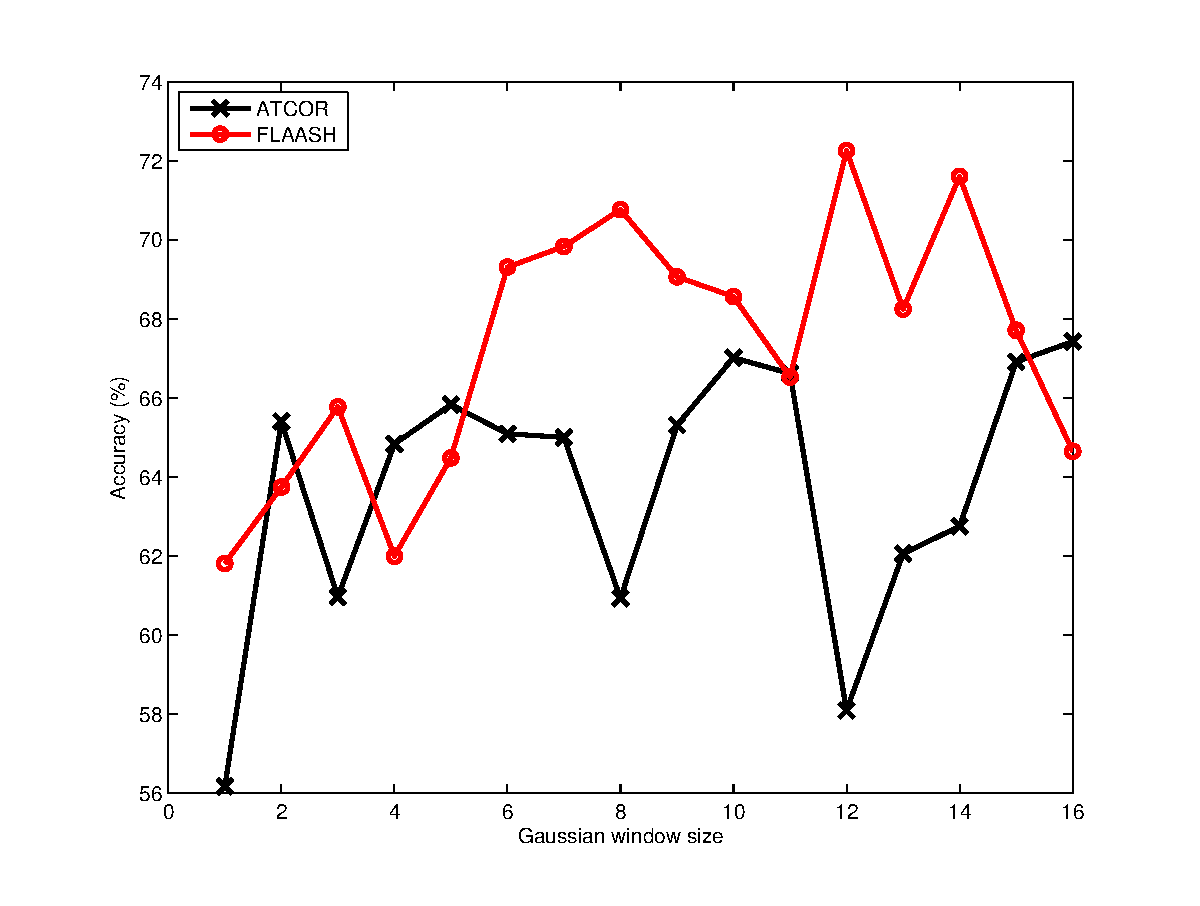
\includegraphics[height=2.5in,keepaspectratio]{./images/after-removing-ndvi-nir.eps}}\hspace{1em}%

   \caption{Impact of Removing low NDVI and NIR pixels}
       \label{fig:after removing NDVI NIR}
\end{figure}


Finally, we look at the effect of atmospheric correction on prediction accuracy vs classification model parameters.
$C, \sigma, P, MaxIter$ and \textit{optimization method} are the knobs of SVM that we tune in a mixture of grid and heuristic search.
$C$ stands for cost or penalty of misclassification against simplicity of the decision surface, $\sigma$ (or also known as $\gamma$ in literature) defines how far the influence of a single training example reaches, with low values meaning 'far' and high values meaning 'close' in RBF function.
$P$ is the polinomial degree for polynomial function as kernel. $MaxIter$ is the maximum number of iterations the optimization function is supposed to run. 
and \textit{optimization method} defines what optimization method we select. 
For parameters except $\sigma$ and $P$ we set $C=+\infty$, $ MaxIter=10,000$ and \textit{optimization method} to quadratic programming. 
In what follows we evaluate the impact of $P$ and $\sigma$ respectively as demonstrated in Figure \ref{fig:parameter tuning}.
 
Figure \ref{fig:parameter tuning:poly} demonstrates the impact of polynomial degree $P$ on prediction accuracy using a polynomial kernel in SVM. 
FLAASH atmospherically corrected data yields 73.5\% of accuracy while ATCOR results in 69.8\%.
The simpler the polinomial, the better the performance; with more complicated polynomial we get a high bias classification model which performs poorly when evaluated on test data.
For FLAASH atmospheric correction with $P \geq 3$ the optimization function does not reach cnvergence in the number of $MaxIter$. 
On the other hand, ATCOR data performs as predicted, the data seems to be showing a linear separability which as the kernel becomes more complex shows signs of overfitting as FLAASH.
Accuracy gets as low as 10.8\% and 11.3\% with polinomila degrees of 7 and 8.

The Radial Basis kernel has better performance yields than polynomial.
As shown in Figure \ref{fig:parameter tuning:RBF}, with a peak at 75.3\% we achieve the best results using FLAASH data while ATCOR comes close at 74.9\%.
RBF does not show good performance at either too low or too high $\sigma$ values.
$\sigma$ is the inverse of the width of the RBF kernel (roughly defining the area of influence of a support vector); 
in other terms, it defines how much influence a single training example has.
The larger $\sigma$ is, the closer other examples must be to be affected.
As RBF takes data to a higher dimentionality, on what $\sigma$ provides:
A small $\sigma$ gives you a pointed bump in the higher dimensions, a large gamma gives you a softer, broader bump.
So neither extreme shows a good fit and a middle point of $\sigma=10,000$ provides best results.
On the negative side, FLAASH begins with an accuracy of 0\% and ATCOR at 19.9\%, but they quickly get to a stable region close by to each other while FLAASH demonstrates superior performance in most of the cases.
There is a good range of $\sigma$ values ($[10, 10000]$) where we reach a somehow plain in prediction accuracy which shows a more robust performance than polynomia. 

% http://tex.stackexchange.com/questions/42968/reduction-of-space-between-two-sub-figures
\begin{figure}[t]
  % Fixed length
  \centering
  \subcaptionbox{Tuning polynomial order for SVM with polynomial kernel function\label{fig:parameter tuning:poly}}{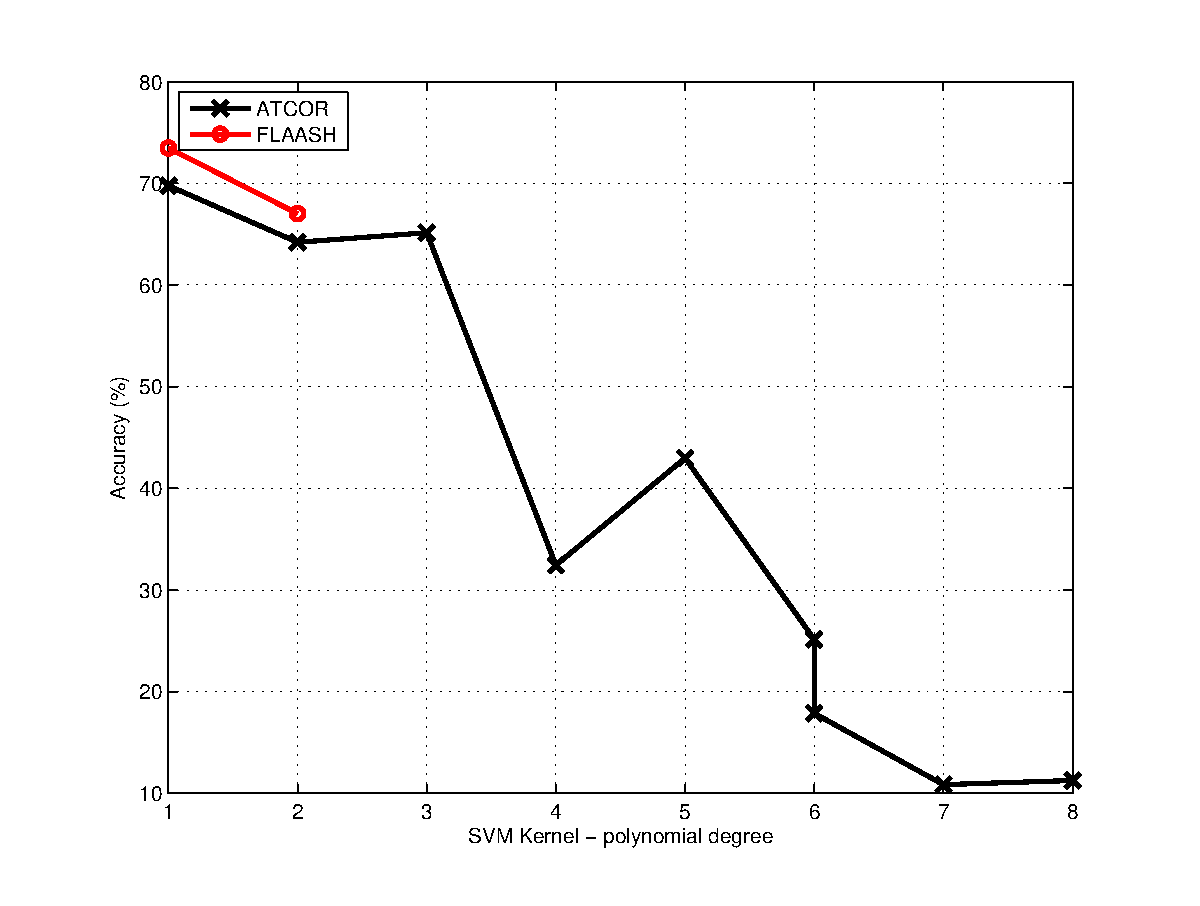
\includegraphics[height=2.5in,keepaspectratio]{./images/poly.eps}}\hspace{1em}%
  \subcaptionbox{Tuning $\sigma$ in SVM with RBF kernel function\label{fig:parameter tuning:RBF}}{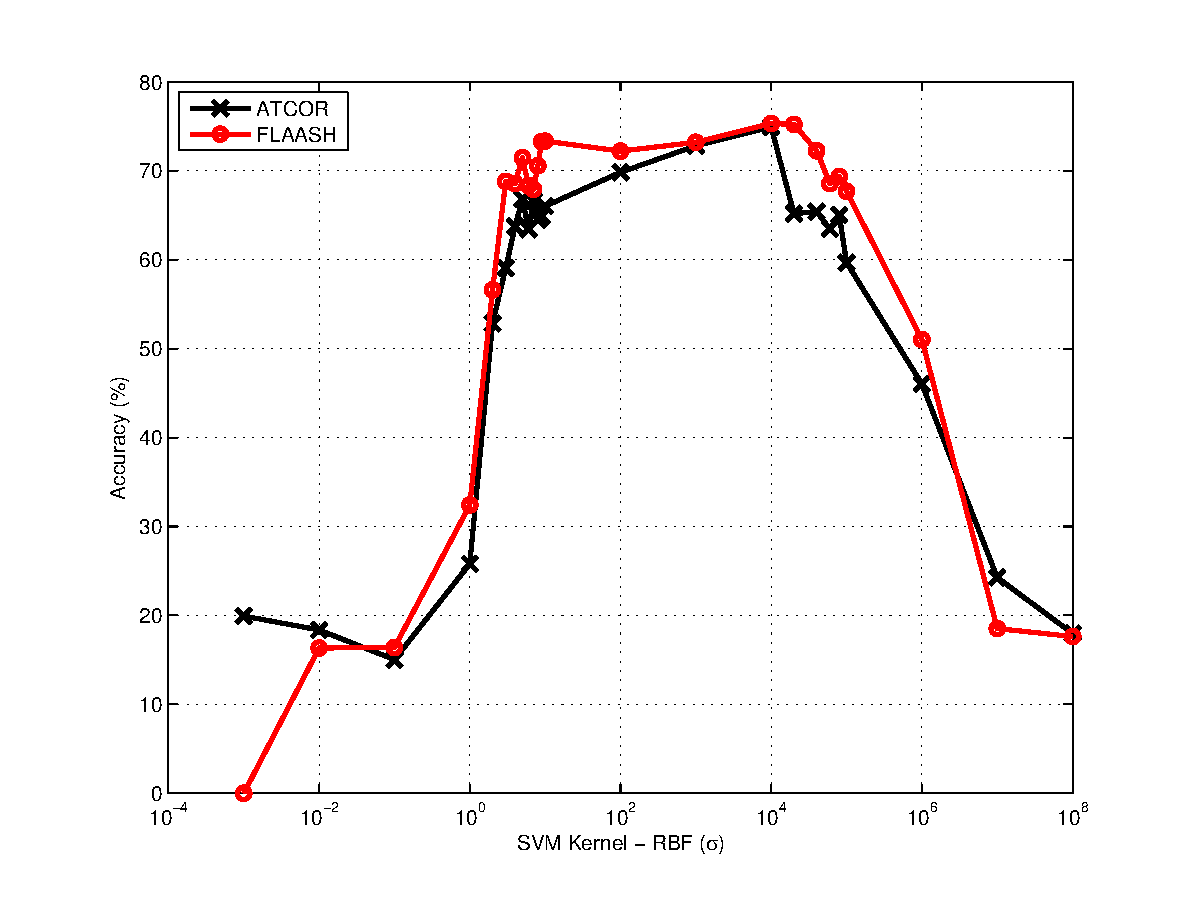
\includegraphics[height=2.5in,keepaspectratio]{./images/rbf.eps}}
   \caption{Parameter tuning for classification algorithms}
       \label{fig:parameter tuning}
\end{figure}



%On robustness of our classification scheme from the Figure \ref{fig:atmospheric correction} and Figure \ref{fig:parameter tuning} you can see that in the box plot, the 25th and 75th percentiles are less than 4\% long in the accuracy axis. 
%This means that our classification is always within $\pm 2$ of the median, and that we are stable in terms of visited ground data. 
%This is further asserted in Figure \ref{fig:robustness}, where even after taking $\frac{2}{3}$ for training and $\frac{1}{3}$ for test, we received similar results as the k-fold scenario with 4\% as the length of 25th-75th percentile. 










% http://tex.stackexchange.com/questions/42968/reduction-of-space-between-two-sub-figures
%\begin{figure}[t]
  % Fixed length
%  \centering
%  \subcaptionbox{Tuning polynomial order for SVM with polynomial kernel function\label{fig:parameter tuning:poly}}{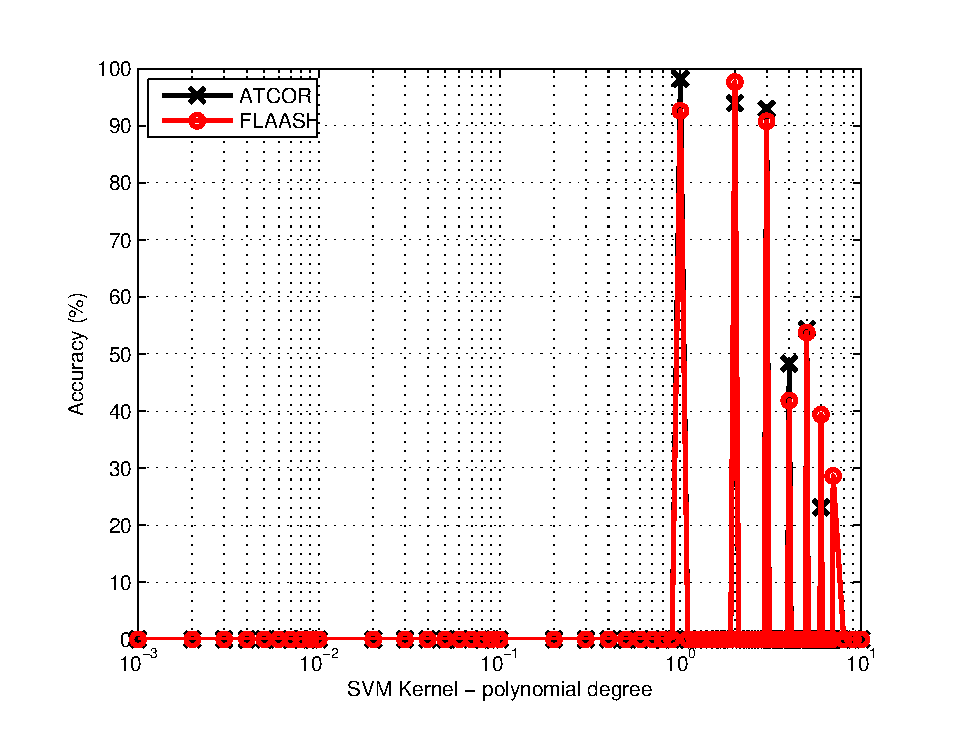
\includegraphics[height=2.5in,keepaspectratio]{./images/atcor_flaash/poly_atcor_flaash.eps}}\hspace{1em}%
%  \subcaptionbox{Tuning $\sigma$ in SVM with RBF kernel function\label{fig:parameter tuning:RBF}}{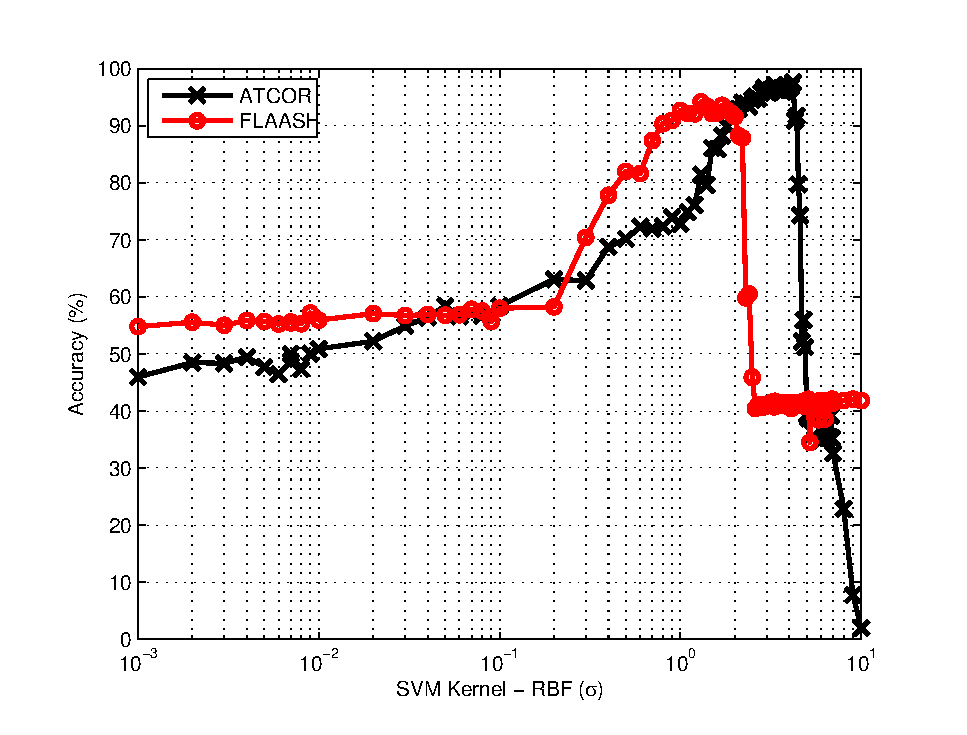
\includegraphics[height=2.5in,keepaspectratio]{./images/atcor_flaash/rbf_atcor_flaash.eps}}
%   \caption{Parameter tuning for classification algorithms}
%       \label{fig:parameter tuning}
%
%\end{figure}



\begin{table}[t]
\begin{center}

\scalebox{0.85}{


\begin{tabular}{lllllllll|}
& & \multicolumn{6}{c}{Predicted Class}                                                                         \\  \cline{3-9}  
                                                                                &                                         & \multicolumn{1}{|c|}{Pine (other)} & \multicolumn{1}{c|}{Longleaf Pine} & \multicolumn{1}{c|}{Turkey Oak} & \multicolumn{1}{c|}{Live Oak} & \multicolumn{1}{c|}{Oak (other)} & \multicolumn{1}{c|}{Laurel Oak} & $\mathbf{\sum}$\\  \cline{2-9} 
\multicolumn{1}{c|}{\multirow{7}{*}{\begin{sideways}Known Class\end{sideways}}} & \multicolumn{1}{c|}{Pine (other)}       & \multicolumn{1}{c|}{10}   & \multicolumn{1}{c|}{10} & \multicolumn{1}{c|}{3}  & \multicolumn{1}{c|}{0}  & \multicolumn{1}{c|}{0} & \multicolumn{1}{c|}{0} & \multicolumn{1}{c|}{23} \\ \cline{2-9}  
\multicolumn{1}{c|}{}                                                           & \multicolumn{1}{c|}{Longleaf Pine}      & \multicolumn{1}{c|}{20}   & \multicolumn{1}{c|}{36} & \multicolumn{1}{c|}{0}  & \multicolumn{1}{c|}{0}  & \multicolumn{1}{c|}{0} & \multicolumn{1}{c|}{4} & \multicolumn{1}{c|}{60}\\ \cline{2-9}  
\multicolumn{1}{c|}{}                                                           & \multicolumn{1}{c|}{Turkey Oak}         & \multicolumn{1}{c|}{1}    & \multicolumn{1}{c|}{0}  & \multicolumn{1}{c|}{62} & \multicolumn{1}{c|}{0}  & \multicolumn{1}{c|}{0} & \multicolumn{1}{c|}{0} & \multicolumn{1}{c|}{63}\\ \cline{2-9} 
\multicolumn{1}{c|}{}                                                           & \multicolumn{1}{c|}{Live Oak}           & \multicolumn{1}{c|}{0}    & \multicolumn{1}{c|}{0}  & \multicolumn{1}{c|}{0}  & \multicolumn{1}{c|}{44} & \multicolumn{1}{c|}{4} & \multicolumn{1}{c|}{0} & \multicolumn{1}{c|}{48}\\ \cline{2-9} 
\multicolumn{1}{c|}{}                                                           & \multicolumn{1}{c|}{Oak (other)}        & \multicolumn{1}{c|}{0}    & \multicolumn{1}{c|}{0}  & \multicolumn{1}{c|}{0}  & \multicolumn{1}{c|}{0}  & \multicolumn{1}{c|}{1} & \multicolumn{1}{c|}{9} & \multicolumn{1}{c|}{10}\\ \cline{2-9} 
\multicolumn{1}{c|}{}                                                           & \multicolumn{1}{c|}{Laurel Oak}         & \multicolumn{1}{c|}{1}    & \multicolumn{1}{c|}{0}  & \multicolumn{1}{c|}{0}  & \multicolumn{1}{c|}{0}  & \multicolumn{1}{c|}{0} & \multicolumn{1}{c|}{5} &  \multicolumn{1}{c|}{6}\\ \cline{2-9} 
\multicolumn{1}{c|}{}                                                           & \multicolumn{1}{c|}{$\mathbf{\sum}$}    & \multicolumn{1}{c|}{32}    & \multicolumn{1}{c|}{46}  & \multicolumn{1}{c|}{65}  & \multicolumn{1}{c|}{44}  & \multicolumn{1}{c|}{5} & \multicolumn{1}{c|}{18} &  \multicolumn{1}{c|}{210}\\ \cline{2-9} 


\end{tabular}
}
 \caption{Demo of confusion matrix using RBF kernel function with accuracy 75.2\% near peak}
    \label{table:confusion matrix}\end{center}
    
\end{table}

Table \ref{table:confusion matrix} demonstrates the confusion matrix of the proposed clasification model at a near peak setup (75.2\%). 
You can see that the majority of missclassifications are between Pine (other) class and Longleaf Pine. 
Similar misclassification can be found between Oak (other) and other types of Oak. 
This is due ot the fact that this class of Oak or Pines is a mixture of different types of Oak or Pine repectively which might include Longleaf Pine or Laurel Oak and such conformance migt be unavoidable. 
The main advantage of this approach is that there is mere misclassification between oak vs Pine category.
The oak category is rarely misclassified as pine, but pines have been mistaken with Turkey Oak and Laurel Oak. 
One should also note that different species of oak are not misclassified to each other. 
Laurel Oak, Turkey Oak and Live Oak are not mistaken for each other, this shows a good intra broad-leaf species classification.  


% http://tex.stackexchange.com/questions/42968/reduction-of-space-between-two-sub-figures
%\begin{figure}[t]
  % Fixed length
%  \centering
%  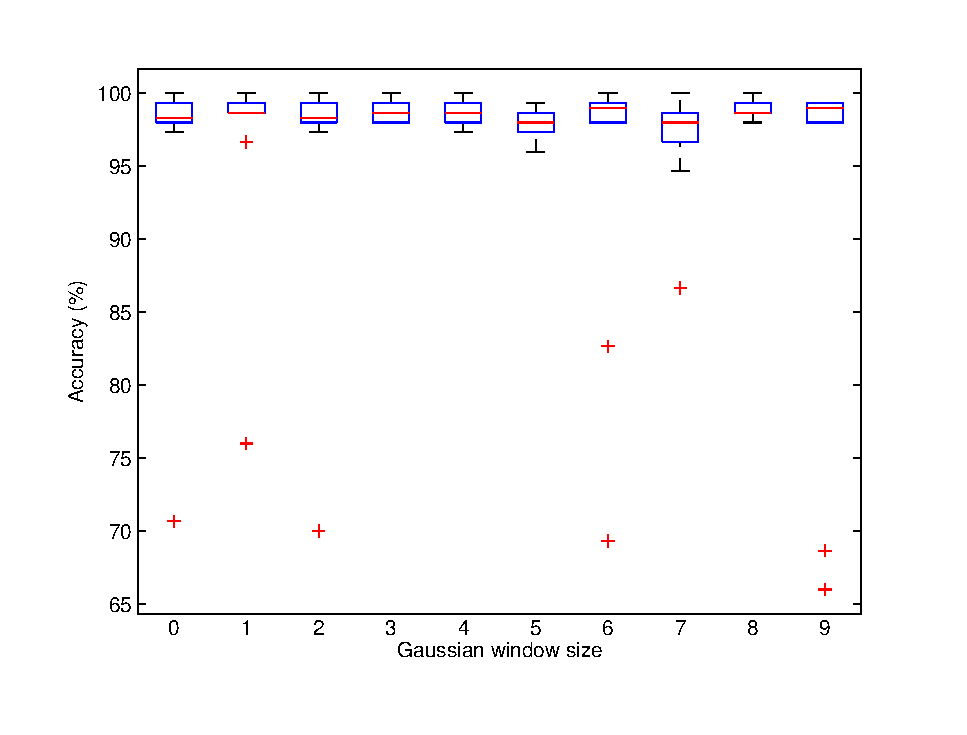
\includegraphics[height=2.5in,keepaspectratio]{./images/atcor_flaash/robustness.eps}
%   \caption{Verifying robustness of classification by applying a $\frac{2}{3}$ training $\frac{1}{3}$ test using polynomial kernel of degree 3}
%       \label{fig:robustness}

%\end{figure}



%\begin{tabular}{|r|c|l|}
%\hline 
%A & B & C \\
%\hline 
%1 & 2 & 3 \\
%\hline 
%\end{tabular}
%\begin{tabular}{|r|c|l|}
%\hline 
%A & B & C \\
%\hline 
%\rule{0pt}{25pt}1 & 2 & 3 \\
%\hline 
%\end{tabular}




% apply ndvi and nir filters to see if any training sets will be removed. 

%\begin{itemize}
%\item \red{Adding Lidar and classification using it}
%\item \red{global predicted maps with legend}
%\item{impact of feature reduction on accuracy before and after lidar}
%\item \red{Mention that the actual neon system will be at higher resolution}
%\item \red{compare airborne reflectance to ground}
%\end{itemize}
%Future works on this project includes a) knowledge reasoning on enhancing mis-classification of Live oak vs Pine b) Add endmember features and verify its utility in enhancing classification accuracy c) Robustness as discussed by Dr. Gader.
% add ground pixel count for related papers
% 
% use hyperspectral library and trying to reduce noise by using lidar
% show ROC curve http://en.wikipedia.org/wiki/Receiver_operating_characteristic
%add user accuracy producer accuracy
% 
% FLAASH reference http://www.exelisvis.com/docs/backgroundflaash.html
% ATCOR reference http://atcor.com/pdf/atcor3_manual.pdf  
% http://www.spectral.com/pdf/sr117.pdf






%% Example of a theorem:
%\begin{Theorem}
%Text text text
%\end{Theorem}

%% Example of a proof:
%\begin{proof}[Proof of Theorem 1]
%Text text text
%\end{proof}


%%%%%%%%%%%%%%%%%%%%%%%%%%%%%%%%%%%%%%%%%%

\section{Conclusions}

Identifying species using remote sensing technologies such as hyperspectral and LiDAR sensors has a critical utility in studying global warming, bio-mass estimation, carbon preserves, invasive species identification and etc. 
In this paper we perform species classification using SVM over AVIRIS hyperspectral data available via NEON from Ordway Swisher Biological Station in north-central Florida.
Our focus is on comparing FLAASH and ATCOR atmospheric corrections while we analize pre-processing techniques both at signal level (Gaussian Filter, Water Absorption Bands Filter) and pixel level (NDVI and NIR Filters).
We found Gaussian Filter and Water Absorption Bands Filter to be helpful in prediction model performance but NDVI and NIR degraded the performance when applied to continous canopies of similar species. 
In all these scenarios we compared FLAASH and ATCOR atmospheric corrections and noted that FLAASH data supersedes ATCOR in majority of the scenarios.
Our model performed robust in intra broad-leaf classification with minor inter conifer/broad-leaf misclassifications.

%\acknowledgements{Acknowledgements}

%This work is supported ...

%%%%%%%%%%%%%%%%%%%%%%%%%%%%%%%%%%%%%%%%%%

% \authorcontributions{Author Contributions}

% Main text.

%%%%%%%%%%%%%%%%%%%%%%%%%%%%%%%%%%%%%%%%%%

%\conflictofinterests{Conflicts of Interest}

%State any potential conflicts of interest here or ``The authors declare no conflict of interest''. 

\bibliography{citation}
\bibliographystyle{mdpi}

\end{document}



